\باب{یکساں حال، برقرار چالو معاصر مشین}
%i have proof read urdu.entire chapter
معاصر مشین وہ گھومنے والی مشین ہے جو ایک مقررہ رفتار سے گھومتی ہے۔ یہ رفتار فراہم کردہ برقی دباو کے تعدد پر منحصر ہوتی ہے۔

کسی جنریٹر پر بوجھ تبدیل کرنے یا جنریٹر کو میکانی طاقت فراہم کرنے والے کی رفتار تبدیل کرنے کے چند ہی لمحات  میں جنریٹر نئی حالات کے  مطابق  دوبارہ برقرار  صورت اختیار کر لیتا ہے۔اس برقرار چالو حال میں اس کی رفتار، برقی دباو، برقی رو، درجہ حرارت وغیرہ  تبدیل نہیں ہوتے ہیں۔اسی طرح  موٹر پر بوجھ تبدیل کرنے سے موٹر کی درکار طاقت اور برقی رو تبدیل ہوں گے۔بوجھ تبدیل ہونے سے قبل موٹر  ایک مستقل برقی رو حاصل کرتی  اور ایک مستقل درجہ حرارت  پر رہتی ہے۔بوجھ تبدیل ہونے کے چند ہی لمحات میں موٹر دوبارہ ایک نئی برقرار چالو صورت اختیار کرتی ہے جہاں اس کا برقی رو ایک نئی قیمت پر برقرار رہتا ہے اور اس کا درجہ حرارت بھی ایک نئی قیمت اختیار کرتا ہے۔دو مختلف برقرار چالو، یکساں صورتوں کے درمیان چند لمحات کے لئے مشین \اصطلاح{عارضی حال}\فرہنگ{حال!عارضی}\حاشیہب{transient state}\فرہنگ{transient state} میں ہوتی ہے۔اس باب میں \اصطلاح{یکساں حال}\فرہنگ{حال!یکساں}\حاشیہب{steady state}\فرہنگ{steady state}، \اصطلاح{برقرار چالو}\فرہنگ{برقرار چالو} معاصر مشین پر تبصرہ کیا جائے گا۔ 

معاصر مشین کے قوی لچھے عموماً ساکن ہوتے ہیں  جبکہ اس کے میدانی لچھے معاصر رفتار سے گھومتے ہیں۔ میدانی لچھوں کا برقی رو قوی لچھوں کے برقی رو کی نسبت  بہت کم ہوتا ہے لہٰذا میدانی لچھوں کو گھمایا جاتا ہے اور ان تک برقی رو سرک چھلوں کے ذریعہ پہنچایا جاتا ہے۔قوی لچھوں کو اس لئے گھومتے حصہ پر نسب نہیں کیا جاتا ہے کہ سرک چھلوں کے ذریعہ ان کا (نسبتاً بہر زیادہ) برقی رو منتقل کرنا مشکل ثابت ہوتا ہے۔یوں قوی لچھوں کو ساکن رکھا جاتا ہے۔

 ہم  دیکھ چکے ہیں کہ تین دوری ساکن لچھوں میں  متوازن تین دوری برقی رو  ایک گھومتے مقناطیسی دباو کی موج پیدا کرتے ہیں۔اس گھومتی موج کی رفتار کو \اصطلاح{معاصر رفتار}\فرہنگ{معاصر رفتار}\حاشیہب{synchronous speed}\فرہنگ{synchronous speed}  کہتے ہیں۔ معاصر مشین کا گھومتا حصہ اسی رفتار سے گھومتا ہے۔ 

معاصر مشین کے میدانی لچھے کو یک سمت  برقی رو درکار ہوتا ہے جو  سرک چھلوں کے ذریعہ اس تک باہر سے پہنچایا جاتا ہے یا  مشین کے دھرے پر  نسب ایک چھوٹے یک سمت  جنریٹر سے  فراہم کیا جاتا ہے۔

میدانی لچھا ایک میدانی مقناطیسی دباو پیدا کرتا ہے جو میدانی لچھے کے ساتھ ساتھ معاصر رفتار سے گھومتا ہے۔ یوں معاصر مشین کے گھومتے لچھوں کی مقناطیسی دباو موج  اور ساکن لچھوں کی مقناطیسی دباو موج معاصر رفتار سے  گھومتی ہیں جس کی بنا  ان مشینوں کو  \اصطلاح{معاصر مشین}\فرہنگ{معاصر!مشین} کہتے ہیں۔

\حصہ{متعدد دوری معاصر مشین}
معاصر مشین عموماً تین دوری ہوتے ہیں۔تین دوری ساکن قوی لچھے خلائی درز میں  \عددیء{120\degree} برقی زاویہ پر نسب ہوتے ہیں جبکہ  میدانی لچھے گھومتے حصے پر نسب ہوتے ہیں اور ان میں یک سمت  برقی رو ہوتا ہے۔ 

مشین کے گھومتے حصے کو بیرونی میکانی طاقت سے گھمانے سے  مشین ایک معاصر جنریٹر کے طور پر کام کرتی ہے اور اس کے تین دوری ساکن قوی لچھوں میں تین دوری برقی دباو پیدا ہو گا جس کا برقی تعدد گھومنے کی رفتار پر منحصر ہو گا۔ اس کے برعکس،  مشین کے تین  دوری ساکن قوی لچھوں کو تین دوری برقی طاقت مہیا کرنے سے مشین ایک معاصر موٹر کے طور پر کام کرتی ہے جو معاصر رفتار سے گھومے گی۔مشین کی کل برقی قوت کے چند فی صد  برابر برقی قوت  میدان لچھے کو درکار ہوتی ہے۔

\begin{figure}
\centering
%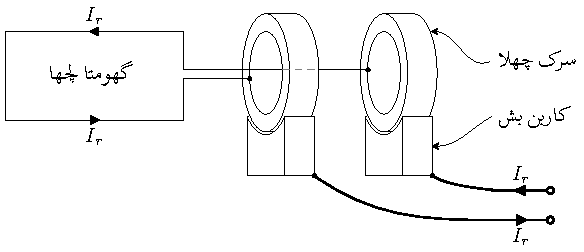
\includegraphics{figSynchronousSlipRings}
\begin{tikzpicture}
%grid
%\draw[gray,thick] (-2*\sRo,-2*\sRo) grid (2*\sRo,3*\sRo);
%\draw[gray,thin,xstep=0.1,ystep=0.1] (-2*\sRo,-2*\sRo) grid (2*\sRo,3*\sRo);
%
\pgfmathsetmacro{\sY}{1}
\pgfmathsetmacro{\sX}{0.4}
\pgfmathsetmacro{\sW}{0.5}
\pgfmathsetmacro{\bH}{1}
\pgfmathsetmacro{\g}{0.05}
\pgfmathsetmacro{\cH}{1.5}
\pgfmathsetmacro{\cW}{3}
\pgfmathsetmacro{\cG}{0.1}
\pgfmathsetmacro{\cArm}{1}
%
\pgfmathsetmacro{\shiftX}{2cm}
%
%SLIP RING
%\draw (0,0) ellipse (\sX cm and \sY cm);        %moved to end to cover part of bush
%\draw (0,0) ellipse (0.7*\sX cm and 0.7*\sY cm);
\draw(\sW,0)++(-90:\sX cm and \sY cm) arc (-90:90:\sX cm and \sY cm);
\draw(0,\sY)--++(\sW,0);
\draw(0,-\sY)--++(\sW,0);
%%BUSH
\path(-135:\sX cm +\g cm and \sY cm+\g cm)++(0,-\bH)coordinate(bushLowerLeft);
\draw[fill=white](-135:\sX cm +\g cm and \sY cm+\g cm)coordinate(arcS) arc (-135:-45:\sX cm +\g cm and \sY cm+\g cm)coordinate(arcE) --++(\sW,0)--++(0,-\bH)coordinate(bushConnectionA)--++(-\sW,0)--(bushLowerLeft)--cycle;
\draw(arcE)--++(0,-\bH);
\draw(arcS)--++(\sW,0);   %this is the invisible side and needs to be covered
%SLIP RING
\draw[fill=white] (0,0) ellipse (\sX cm and \sY cm);   %shade a portion of the bush
\draw (0,0) ellipse (0.7*\sX cm and 0.7*\sY cm);
%ONE TURN COIL
\draw (0,0)++(0,\cG/2)coordinate(coilS) --++(-\cArm-\sX,0)--++(0,\cH/2-\cG) to [short,i_={$I_r$}] ++(-\cW,0)--++(0,-\cH)  to [short,i_={$I_r$}] ++(\cW,0)--++(0,\cH/2-\cG/2)--++(\cArm+0.13,0)coordinate(coilE);
\draw[fill] (coilE) circle (1pt);
\draw(coilS)--++(0.29,0)coordinate(coilSS);
\draw[gray,dashed] (coilSS)--++(\sW+0.1,0)coordinate(coilSSS);
%\draw(coilSSS)--++(1 cm,0);    %gets covered by the second slip ring so moved to end
%
%external wire to bush
\draw[fill] (bushConnectionA) circle (1pt);
\draw[thick] (bushConnectionA) to [out=-35,in=180] ++(3,-0.75)coordinate(negCon) to [short,i_={$I_r$,-o}]++(1,0);
%urdu text
\draw node at (-3,0){\RL{گھومتا لچھا}};
%===============
\begin{scope}[xshift=\shiftX]
%\draw[gray,thick](-2,-2) grid (2,2);
%\draw[gray,thin,xstep=0.1,ystep=0.1](-2,-2) grid (2,2);
%SLIP RING
\draw(\sW,0)++(-90:\sX cm and \sY cm) arc (-90:90:\sX cm and \sY cm);
\draw(0,\sY)--++(\sW,0);
\draw(0,-\sY)--++(\sW,0);
%BUSH
\path(-135:\sX cm +\g cm and \sY cm+\g cm)++(0,-\bH)coordinate(bushLowerLeft);
\draw[fill=white](-135:\sX cm +\g cm and \sY cm+\g cm)coordinate(arcS) arc (-135:-45:\sX cm +\g cm and \sY cm+\g cm)coordinate(arcE) --++(\sW,0)--++(0,-\bH)coordinate(bushConnectionB)--++(-\sW,0)--(bushLowerLeft)--cycle;
\draw(arcE)--++(0,-\bH);
\draw(arcS)--++(\sW,0);   %this is the invisible side and needs to be covered
%SLIP RING
\draw[fill=white] (0,0) ellipse (\sX cm and \sY cm);   %shade a portion of the bush
\draw (0,0) ellipse (0.7*\sX cm and 0.7*\sY cm);
%external wire to bush
\draw[fill] (bushConnectionB) circle (1pt);
\draw[thick] (bushConnectionB) to [out=-35,in=0] ++(1,-0.25) to [short,i<={$I_r$},-o]++(1,0);

\draw[stealth-](0.8,0.7) to [out=0,in=210] ++(1,-0.5)node[right]{\RL{سرک چھلا}};
\end{scope}
%
\draw(coilSSS)--++(0.84 cm,0)coordinate(coilSSSS);
\draw[fill] (coilSSSS) circle (1pt) ;
%urdu text
\draw[stealth-] (bushConnectionB)++(0,\bH/2) to [out=0,in=210] ++(1,0.5)node[right]{\RL{کاربن بش}};
\end{tikzpicture}%
\caption{کاربن بُش اور سرک چھلوں کے ذریعہ گھومتے لچھے تک برقی رو پہنچایا گیا ہے۔}
\label{شکل_معاصر_سرک_چھلے}
\end{figure}


 گھومتے لچھے تک برقی دباو مختلف طریقوں سے پہنچایا جا سکتا ہے۔شکل \حوالہ{شکل_معاصر_سرک_چھلے}  میں گھومتے لچھے تک موصل \اصطلاح{سرک چھلے}\فرہنگ{سرک چھلے}\حاشیہب{slip rings}\فرہنگ{slip rings}  کی مدد سے یک سمت  برقی رو پہنچانے کا طریقہ دکھایا گیا ہے۔  سرک چھلے اسی دھرے  پر نسب ہوں گے جس پر گھومتا لچھا نسب ہو گا لہٰذا سرک چھلے اور  گھومتے لچھے ایک ہی رفتار سے حرکت کریں گے۔

کاربن کے ساکن بش، اسپرنگ  کی مدد  سے، سرک چھلوں  کی بیرونی سطح  کے ساتھ دبا کر رکھے جاتے ہیں۔ جب مشین چلتی ہے،  کاربن بش ان سرک چھلوں پر سرکتے ہیں۔ اسپرنگ کا دباو ان کا برقی جوڑ مضبوط رکھتا ہے تا کہ ان کے بیچ چنگاریاں نہ نکلیں۔ کاربن بش کے ساتھ برقی تار جڑی ہے۔  یک سمت  برقی رو \عددیء{I_r} ، کاربن بش\فرہنگ{کاربن بش}\فرہنگ{بش}\حاشیہب{carbon bush}\فرہنگ{carbon bush} اور سرک چھلوں  سے ہوتا ہوا،  گھومتے لچھے تک پہنچتا ہے۔

بڑی معاصر مشین کا میدانی یک سمت  رو عموماً  ایک چھوٹے بدلتا رو جنریٹر سے حاصل کیا جاتا ہے جو معاصر مشین کے دھرے پر  نسب ہوتا ہے اور دھرے  کے ساتھ  گھومتا ہے۔ چھوٹے جنریٹر کے برقی دباو کو دھرے پر  نسب برقیاتی سمت کار کی مدد سے یک سمت  برقی دباو میں تبدیل کیا جاتا ہے۔ یوں سرک چھلے کی ضرورت پیش نہیں آتی ہے۔سرک چھلے بوجہ  رگڑ خراب ہوتے ہیں جس کی وجہ سے معاصر مشین کی مرمت درکار ہوتی ہے جو  ایک مہنگا کام ہے۔اسی لئے چھوٹا  جنریٹر استعمال کرتے ہوئے سرک چھلوں سے نجات حاصل کی جاتی ہے۔

اُبھرے قطب\فرہنگ{قطب!ابھرے}\حاشیہب{salient poles} مشین، پانی سے چلنے والے سست رفتار جنریٹر اور  عام استعمال کی موٹروں کے لئے موزوں  ہیں جبکہ ہموار قطب\فرہنگ{قطب!ہموار}\حاشیہب{non-salient poles}\فرہنگ{non-salient poles} مشین، تیز رفتار دو یا چار قطبی \اصطلاح{چرخاب}\فرہنگ{چرخاب}\حاشیہب{turbine}\فرہنگ{turbine} جنریٹروں کے لئے موزوں  ہیں۔

ایک (بڑی) سلطنت کو درکار برقی توانائی  کسی ایک  جنریٹر سے پیدا کرنا ممکن نہیں ہوتا ہے بلکہ چند درجن سے لے کر کئی سو  جنریٹر بیک وقت یہ فریضہ سرانجام دیتے  ہیں۔ ایک سے زیادہ جنریٹر استعمال کرنا فائدہ مند ثابت ہوتا ہے۔ اول، برقی توانائی کی ضرورت کے مطابق جنریٹر چالو کئے جا سکتے ہیں۔ دوم،  جنریٹروں کو ان مقامات کے قریب نسب کیا جا سکتا ہے جہاں جہاں برقی توانائی درکار ہو۔ اس طرح کے بڑے نظام میں ایک جنریٹر کی حیثیت بہت کم ہوتی ہے لہٰذا کسی ایک جنریٹر کو چالو یا بند کرنے سے پورے نظام پر کوئی خاص اثر نہیں پڑتا ہے۔ یوں ہم سلطنت کے برقی نظام کو ایک مقررہ برقی دباو اور ایک مقررہ برقی تعدد کا لامتناہی نظام تصور کر سکتے ہیں۔ معاصر جنریٹر کو لامتناہی نظام کے ساتھ جڑا تصور کر کے معاصر جنریٹر کے کئی اہم پہلو با آسانی سمجھے جا سکتے ہیں۔

مساوات \حوالہ{مساوات_گھومتے_مشین_مروڑ_اور_بہاو}   معاصر مشین کی قوت مروڑ دیتی ہے۔اس مساوات کے مطابق برقی قوت مروڑ، مشین میں موجود متعامل مقناطیسی دباو کو ایک دوسرے کی سیدھ میں لانے کی کوشش کرتی ہے۔ برقرار  چالو  مشین کی  برقی قوت مروڑ اور مشین کے دھرے پر لاگو میکانی قوت مروڑ ایک دوسرے کے برابر ہوتی ہیں۔ جب مشین ایک جنریٹر کی حیثیت سے استعمال ہو تب میکانی طاقت  دھرے کو گھماتا ہے اور گھومتے لچھے کا مقناطیسی دباو کُل مقناطیسی دباو سے گھومنے کے رخ  آگے ہوتا ہے۔ مساوات \حوالہ{مساوات_گھومتے_مشین_مروڑ_اور_بہاو} سے حاصل قوت مروڑ ایسی صورت میں مشین کو گھومنے سے روکنے کی کوشش کرتا ہے۔میکانی طاقت چلتے پانی، ایندھن سے چلتے انجن، وغیرہ سے حاصل ہو سکتا ہے۔ اسی طرح اگر مشین ایک موٹر کی حیثیت سے استعمال ہو، تب صورت اس کے بالکل اُلٹ ہو گی۔

کل مقناطیسی بہاو  \عددیء{\phi_{ar}} اور گھومتے لچھے کا مقناطیسی دباو \عددیء{\tau_r} تبدیل نہ ہونے کی صورت میں  مساوات \حوالہ{مساوات_گھومتے_مشین_مروڑ_اور_بہاو} کے مطابق مشین کی قوت مروڑ  \عددیء{\sin \theta_r} کے ساتھ تبدیل ہو گی۔ اگر زاویہ \عددیء{\theta_r} صفر ہو تب  قوت مروڑ بھی صفر ہو گی۔ اب  تصور کریں کہ یہ مشین ایک موٹر کے طور پر استعمال ہو رہی ہے۔ جیسے جیسے موٹر پر لدا میکانی بوجھ بڑھایا جاتا ہے ویسے ویسے اس کے دھرے پر میکانی قوت مروڑ بڑھے گی۔ موٹر اس زاویہ کو بڑھا بڑھا کر برابر کی برقی قوت مروڑ پیدا کرے گی۔یہاں یہ سمجھنا ضروری ہے کہ موٹر ہر وقت معاصر رفتار سے گھومتی ہے ماسوائے ان لمحات کے لئے جن کے دوران موٹر آہستہ یا تیز  ہو کر زاویہ کو ضرورت کے مطابق درست کرتی ہے۔یعنی موٹر کا زاویہ \عددیء{\theta_r} ہر وقت میکانی قوت مروڑ کا تعقب\فرہنگ{تعقب}\حاشیہب{hunting}\فرہنگ{hunting}  کرتا ہے۔

موٹر پر لدا میکانی بوجھ بتدریج بڑھانے سے ایک لمحہ آئے گا  جب زاویہ \عددیء{\theta_r} نوے درجہ،  \عددیء{\tfrac{\pi}{2}} ریڈیئن، تک پہنچتا ہے۔ اس لمحہ موٹر اپنی انتہائی قوت مروڑ\فرہنگ{قوت مروڑ!انتہائی}\حاشیہب{pull out torque}\فرہنگ{torque!pull out}  پیدا کرے  گی۔ موٹر کسی بھی صورت میں اس سے زیادہ قوت مروڑ پیدا نہیں کر سکتی ہے لہٰذا  بوجھ  مزید بڑھانے سے موٹر رکھ جائے گی۔ ہم کہتے ہیں کہ موٹر نے \اصطلاح{غیر معاصر}\فرہنگ{غیر معاصر}\حاشیہب{lost synchronism} صورت اختیار کر لی ہے۔ مساوات \حوالہ{مساوات_گھومتے_مشین_مروڑ_اور_بہاو} سے ظاہر ہے کہ ایک قطب کا کل مقناطیسی بہاو یا (اور) گھومتے لچھے کا مقناطیسی دباو بڑھا کر موٹر کی  انتہائی قوت مروڑ  بڑھائی جا سکتی ہے۔

یہی صورت  حال اگر مشین برقی جنریٹر کے طور پر استعمال کی جائے سامنے آتی ہے۔ جب بھی مشین غیر معاصر صورت اختیار کرے،  اسے جلد خود کار  \اصطلاح{دور شکن}\فرہنگ{دور شکن}\حاشیہب{circuit breaker}\فرہنگ{circuit breaker} کی مدد سے برقی بھم  رسانی سے الگ کر دیا جاتا ہے۔

ہم نے دیکھا کہ ایک معاصر موٹر صرف اور صرف معاصر رفتار سے ہی گھوم سکتی ہے اور صرف اسی رفتار پر گھوم کر قوت مروڑ پیدا کر سکتی ہے لہٰذا ساکن معاصر موٹر کو  چالو  کرنے کی کوشش  ناکام ہو گی۔ معاصر موٹر کو پہلے کسی دوسرے طریقے سے معاصر رفتار تک لایا جاتا ہے اور اس کے بعد  اسے چالو کیا جاتا ہے۔ ایسا عموماً ایک چھوٹی \اصطلاح{امالی موٹر}\حاشیہب{induction motor}  کی مدد سے کیا جاتا ہے جو بے بوجھ معاصر موٹر کو  معاصر رفتار تک پہنچاتی  ہے جس کے بعد معاصر موٹر کو چالو کیا جاتا ہے۔ ایسی امالہ موٹر عموماً معاصر موٹر کے دھرے پر نسب ہوتی ہے۔

\حصہ{معاصر مشین کے امالہ}
 ہم تصور کرتے ہیں کہ مشین دو قطب اور تین دوری ہے اور اس کے لچھے ستارہ نما جڑے  ہیں۔اس طرح لچھوں میں برقی رو، تار برقی رو\حاشیہب{line current} ہی ہو گا اور ان پر لاگو برقی دباو، یک دوری برقی دباو ہو گا۔ایسا کرنے سے مسئلے پر غور کرنا آسان  اور نتیجہ کسی بھی موٹر کے لئے درست ہوتا ہے۔

شکل \حوالہ{شکل_معاصر_تین_دور_دو_قطب}  میں ایک ایسی تین دوری دو قطبی معاصر مشین دکھائی گئی ہے۔ اس کا گھومتا حصہ نلکی نما ہے۔اس کو دو قطبی مشین یا  \عددیء{P} قطبی مشین کے دو قطبین کا حصہ تصور کیا جا سکتا ہے۔

 اگرچہ یہاں گچھ لچھے دکھائے گئے ہیں، حقیقت میں پھیلے لچھے  استعمال ہوں گے لہٰذا انہیں  پھیلے لچھے تصور کریں۔ اس طرح ہر لچھا سائن نما برقی دباو پیدا کرتا ہے جس کی چوٹی لچھے کی مقناطیسی محور کے رخ ہو گی۔  چونکہ معاصر مشین کے گھومتے لچھے میں یک سمت  رو ہوتا ہے لہٰذا، جیسا شکل \حوالہ{شکل_معاصر_تین_دور_دو_قطب} میں دکھایا گیا ہے، اس لچھے  کا مقناطیسی دباو ہر لمحہ گھومتے حصہ کی مقناطیسی محور کے رخ ہو گا۔ گھومتے لچھے کا مقناطیسی دباو گھومتے حصہ کے ساتھ ساتھ معاصر رفتار سے گھومے گا۔

فرض کریں  کہ یہ مشین معاصر رفتار \عددیء{\omega} سے گھوم رہی ہے۔ یوں  اگر لمحہ \عددیء{t=0} پر دور  \عددیء{a} اور گھومتے لچھے کی مقناطیسی محور کے رخ ایک دوسرے جیسے ہوں تب  کسی بھی لمحہ \عددیء{t} پر ان کے بیچ زاویہ \عددیء{\theta=\omega t} ہو گا۔
\begin{figure}
\centering
%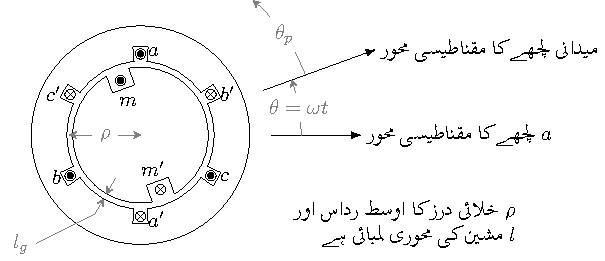
\includegraphics{figSynchronousThreePhaseTwoPole}
\begin{tikzpicture}
%grid
%\draw[gray,thick] (-2*\sRo,-2*\sRo) grid (2*\sRo,3*\sRo);
%\draw[gray,thin,xstep=0.1,ystep=0.1] (-2*\sRo,-2*\sRo) grid (2*\sRo,3*\sRo);
%STATOR
\stator{6}{30}
\slotDot{90,210,330}
\slotCross{-90,-210,-330}
\slotName{90/a/right,210/b/left,330/c/right}
\slotName{-90/a'/right,-210/c'/left,-330/b'/right}
%ROTOR
\pgfmathsetmacro{\pTheta}{160}
\pgfmathsetmacro{\pX}{0}
\pgfmathsetmacro{\pY}{0.3}
\pgfmathsetmacro{\pTilt}{20}
\rotor{2}{\pTilt}
%dot
\draw (90+\pTilt:\rR-2/3*\delR) circle (2.5pt);
\draw[fill] (90+\pTilt:\rR-2/3*\delR) circle (1.5pt);
%cross
\draw (-90+\pTilt:\rR-2/3*\delR) circle (2.5pt);
\draw (-90+\pTilt:\rR-2/3*\delR)++(45:2.2pt)--++(-135:4.4pt);
\draw (-90+\pTilt:\rR-2/3*\delR)++(-45:2.2pt)--++(135:4.4pt);
%rotor name
\draw (90+\pTilt:\rR-2.2*\delR) node {$m$};
\draw (-90+\pTilt:\rR-2.2*\delR) node {$m'$};
%arrows
\draw[-latex](\pTilt:1.2*\sRo)--++(\pTilt:2cm) node[right] {\RL{میدانی لچھے کی مقناطیسی محور}};
\draw[-latex](0:1.2*\sRo)--++(0:1.5 cm)node[right] {\RL{$a$ لچھے کی مقناطیسی محور}};
\draw node[align=right,right] at (2.5,-1.5){\RL{$\rho$ خلائی درز کا اوسط رداس اور} \\ \RL{$l$ مشین کی محوری لمبائی ہے}};
\draw[-stealth](0:1.2*\sRo)++(0:0.5cm) arc (0:\pTilt:1.2*\sRo cm+0.5cm);
\draw(\pTilt/2:1.2*\sRo cm+0.5cm) node[fill=white,xshift=2ex]{$\theta=\omega t$};
\draw[-stealth](\pTilt:1.2*\sRo cm+0.75cm) arc (\pTilt:\pTilt+30:1.2*\sRo cm +0.75 cm);
\draw (\pTilt+15:1.2*\sRo cm +0.75 cm) node[fill=white]{$\theta_p$};
%text
\draw[stealth-stealth](0,0)--++(180:\rR+\gap/2)node[pos=0.5,fill=white]{$\rho$};
\draw[stealth-] (240:\rR)--++(60:0.3 cm);
\draw[stealth-] (240:\rR+\gap)--++(240:0.3 cm)--+(-1,-0.5)node[left]{$l_g$};
\end{tikzpicture}%
\caption{تین دوری، دو قطبی معاصر مشین۔}
\label{شکل_معاصر_تین_دور_دو_قطب}
\end{figure}
امالہ کا ریاضی حساب کرنے کے لئے شکل \حوالہ{شکل_معاصر_تین_دور_دو_قطب}  سے رجوع کریں جہاں  محیط پر خلائی درز یکساں ہے۔ رداسی رخ خلائی  درز  کی  لمبائی \عددیء{l_g} ہے۔ساکن حصے میں شگافوں کے اثر کو نظرانداز کریں۔محور سے خلائی درز تک کا اوسط رداسی فاصلہ \عددیء{\rho} ہے اور مشین کی   محوری لمبائی (دھرے کے رخ) \عددیء{l} ہے۔

کسی بھی لچھے کے خود امالہ کا حساب کرتے وقت باقی تمام لچھوں کو نظرانداز کریں۔یوں  باقی تمام لچھوں میں برقی رو صفر تصور کریں، یعنی ان لچھوں  کے سرے آزاد رکھیں۔ کسی ایک لچھے کے خود امالہ کو پیما سے ناپتے وقت بھی باقی تمام لچھوں کے سرے آزاد رکھیں جائیں گے۔ 


\جزوحصہ{خود امالہ}
گھومتے یا ساکن لچھے کا خود امالہ \عددیء{L} زاویہ \عددیء{\theta} پر منحصر نہیں ہو گا۔ ان میں سے کسی بھی لچھے کا مقناطیسی دباو  \عددیء{\tau}
\begin{align}
\tau=k_w \frac{4}{\pi}\frac{N i}{2} \cos \theta_p
\end{align}
خلائی درز میں درج ذیل  کثافت مقناطیسی بہاو \عددیء{B}  پیدا کرے گا جہاں \عددی{\theta_p} لچھے کے محور سے ناپا جائے گا۔	
\begin{align}
B=\mu_0 H=\mu_0 \frac{\tau}{l_g}=\mu_0 k_w \frac{4}{\pi}\frac{N i}{2 l_g} \cos \theta_p
\end{align}
یہ مساوات زاویہ \عددیء{\theta_p} کے ساتھ  کثافت مقناطیسی دباو \عددیء{B} کا تعلق پیش کرتی ہے۔ لچھا کے ایک قطب پر  کل مقناطیسی بہاو \عددیء{\phi}  اس مساوات کا سطحی تکمل\فرہنگ{سطحی تکمل}\حاشیہب{surface integral}دے گا۔
\begin{gather}
\begin{aligned}\label{مساوات_معاصر_بہاو_بذریع_سطحی_تکمل}
\phi&=\int \kvec{B} \cdot \dif \kvec{S}\\
&=\int_{-\frac{\pi}{2}}^{+\frac{\pi}{2}} B l \rho \dif \theta_p\\
&=\mu_0 k_w \frac{4}{\pi}\frac{N i}{2 l_g} l \rho \int_{-\frac{\pi}{2}}^{+\frac{\pi}{2}}  \cos  \theta_p \dif \theta_p\\
&=\frac{4 \mu_0 k_w N i l \rho}{\pi l_g}
\end{aligned}
\end{gather}
ایک  لچھے کا خود امالہ \عددیء{L}،  مساوات \حوالہ{مساوات_مقناطیسی_دور_خود_امالہ_تعریف} میں جزو پھیلاو \عددیء{k_w} کا اثر  شامل کرتے ہوئے  حاصل کرتے ہیں۔
\begin{align}
L=\frac{\lambda}{i}=\frac{k_w N \phi}{i}=\frac{4 \mu_0 k_w^2 N^2  l \rho}{\pi l_g}
\end{align}
یہ مساوات شکل \حوالہ{شکل_معاصر_تین_دور_دو_قطب} میں تینوں قوی لچھوں کا خود امالہ
\begin{align}\label{مساوات_معاصر_تین_ساکن_امالہ_برابر}
L_{aa0}=L_{bb0}=L_{cc0}=\frac{4 \mu_0 k_{wa}^2 N_a^2  l \rho}{\pi l_g}
\end{align}
اور  میدانی لچھے کا خود امالہ دیتی ہے۔
\begin{align}
L_{mm0}=\frac{4 \mu_0 k_{wm}^2 N_m^2  l \rho}{\pi l_g}
\end{align}

\جزوحصہ{مشترکہ امالہ}
اب ہم دو لچھوں کا مشترکہ امالہ حاصل کرتے ہیں۔تصور کریں صرف  گھومتا لچھا مقناطیسی بہاو پیدا کر رہا ہے۔ ہم  بہاو کے اس حصہ سے، جو \عددیء{a} لچھا  سے گزرتا ہے، گھومتے لچھا اور \عددی{a} لچھا  کا مشترکہ امالہ حاصل کرتے ہیں ۔شکل \حوالہ{شکل_معاصر_تین_دور_دو_قطب}  میں گھومتے اور \عددیء{a} لچھا کے بیچ زاویہ \عددیء{\theta} ہے۔ایسی صورت میں  \عددیء{(-\tfrac{\pi}{2}-\theta)< \theta_p < (\tfrac{\pi}{2}-\theta)} کے بیچ بہاو، \عددیء{a} لچھا سے گزرے گا۔ اس مقناطیسی بہاو کا حساب مساوات \حوالہ{مساوات_معاصر_بہاو_بذریع_سطحی_تکمل}  میں تکمل کی حدیں تبدیل کر کے حاصل کرتے ہیں۔
\begin{gather}
\begin{aligned}
\phi_{am}&=\int \kvec{B} \cdot \dif \kvec{S}\\
&=\int_{-\frac{\pi}{2}-\theta}^{+\frac{\pi}{2}-\theta} B l \rho \dif \theta_p\\
&=\mu_0 k_{wm} \frac{4}{\pi}\frac{N_m i_m}{2 l_g} l \rho \int_{-\frac{\pi}{2}-\theta}^{+\frac{\pi}{2}-\theta} \cos \theta_p \dif \theta_p\\
&=\frac{4 \mu_0 k_{wm}  N_m i_m l \rho}{\pi l_g} \cos \theta
\end{aligned}
\end{gather}
یوں گھومتے لچھا اور \عددی{a} لچھا کا  مشترکہ امالہ
\begin{align}
L_{am}=\frac{\lambda_{am}}{i_m}=\frac{k_{wa} N_a \phi_{am}}{i_m}=\frac{4 \mu_0 k_{wa} k_{wm} N_a N_m l \rho}{\pi l_g} \cos \theta
\end{align}
یا
\begin{align}\label{مساوات_معاصر_ساکن_گھومتا_مشترکہ_امالہ}
L_{am}=L_{am0} \cos \theta
\end{align}
ہو گا جہاں
\begin{align}
L_{am0}=\frac{4 \mu_0 k_{wa} k_{wm} N_a N_m l \rho}{\pi l_g} 
\end{align}
ہے اور \عددیء{\theta=\omega t}  گھومنے کی رفتار پر منحصر ہو گا۔ اگرچہ مساوات \حوالہ{مساوات_معاصر_ساکن_گھومتا_مشترکہ_امالہ} ایک گھومتے اور ایک ساکن لچھے کے لئے حاصل کی گئی  ہے،  درحقیقت یہ  شکل \حوالہ{شکل_معاصر_تین_دور_دو_قطب} میں کسی بھی دو لچھوں کے لئے درست ہے۔  دونوں لچھوں کو ساکن یا دونوں کو متحرک تصور کر کے بھی یہی نتیجہ حاصل ہو گا۔  یوں  دو ساکن  یکساں لچھے، مثلاً \عددیء{a} اور \عددیء{b} جن کے بیچ  \عددیء{120\degree} زاویہ ہے،  کا  مشترکہ امالہ
\begin{align}
L_{ab}&=\frac{4 \mu_0 k_{wa} k_{wb} N_a N_b l \rho}{\pi l_g} \cos 120\degree=-\frac{2 \mu_0 k_{wa}^2  N_a^2 l \rho}{\pi l_g}
\end{align}
ہو گا جہاں یکسانیت کی  بدولت  \عددیء{k_{wb}=k_{wa}} اور \عددیء{N_b=N_a} لئے گئے ہیں۔اگر تینوں ساکن لچھے بالکل یکساں ہوں  تب درج بالا مساوات اور مساوات \حوالہ{مساوات_معاصر_تین_ساکن_امالہ_برابر} کی مدد سے درج ذیل  لکھا جا سکتا ہے۔ 
\begin{align}\label{مساوات_معاصر_ساکن_مشترکہ_امالہ}
L_{ab}=L_{bc}=L_{ca}=-\frac{L_{aa0}}{2}
\end{align}
%
\جزوحصہ{معاصر امالہ}
مشین پر لاگو برقی دباو کو مشین کے لچھوں کا خود امالہ، مشترکہ امالہ اور لچھوں کے برقی رو کی مدد سے لکھا جا سکتا ہے۔ یہ کرنے کے لئے ہم پہلے  لچھوں کی ارتباط بہاو \عددیء{\lambda} کو ان کے امالہ اور برقی رو کی مدد سے لکھتے ہیں۔
\begin{gather}
\begin{aligned}\label{مساوات_معاصر_ارتباط_چار}
\lambda_a&=L_{aa} i_a+L_{ab} i_b +L_{ac} i_c+L_{am} I_m\\
\lambda_b&=L_{ba} i_a+L_{bb} i_b +L_{bc} i_c+L_{bm} I_m\\
\lambda_c&=L_{ca} i_a+L_{cb} i_b +L_{cc} i_c+L_{cm} I_m\\
\lambda_m&=L_{ma} i_a+L_{mb} i_b +L_{mc} i_c+L_{mm} I_m
\end{aligned}
\end{gather}
ان مساوات میں ساکن لچھوں کا بدلتا رو  چھوٹے حروف \عددیء{i_a,i_b,i_c}  جبکہ گھومتے میدانی لچھے کا یک سمت   رو  بڑے حرف  \عددیء{I_m} سے ظاہر کیا گیا ہے۔

ان چار مساوات میں سے ہم کسی ایک کو  حل کرتے ہیں۔ چونکہ چاروں مساوات ایک طرح کی ہیں لہٰذا  باقی بھی اسی طرح حل ہوں گی۔ ہم ان میں  پہلی  مساوات منتخب کرتے ہیں:
\begin{align}\label{مساوات_معاصر_ارتباط_الف_کل}
\lambda_a&=L_{aa} i_a+L_{ab} i_b +L_{ac} i_c+L_{am} I_m
\end{align}
 مساوات \حوالہ{مساوات_معاصر_تین_ساکن_امالہ_برابر}  لچھا  \عددیء{a}  کا خود امالہ دیتی ہے اور اس کو حاصل کرتے ہوئے تصور کیا گیا کہ لچھے کا پورا مقناطیسی بہاو خلائی درز سے گزرتا ہے۔ حقیقت میں ایسا نہیں ہوتا ہے اور مقناطیسی بہاو  کا کچھ حصہ خلائی درز  سے گزر کر دوسری جانب نہیں پہنچ پاتا ہے بلکہ خلائی درز میں رہتے ہوئے لچھے کے گرد چکر کا کچھ حصہ مکمل کرتا ہے۔  مقناطیسی بہاو کا یہ حصہ  \اصطلاح{رستا امالہ}\فرہنگ{امالہ!رستا}\حاشیہب{leakage inductance}\فرہنگ{inductance!leakage} \عددیء{L_{al}}  پیدا کرتا ہے جو  ٹرانسفارمر کے رستا امالہ کی طرح ہوتا ہے۔ یوں لچھے کا کل خود امالہ \عددیء{L_{aa}}  دو حصوں پر مشتمل ہو گا:
\begin{align}\label{مساوات_معاصر_الف_خود_کل_امالہ}
L_{aa}=L_{aa0}+L_{al}
\end{align}
ہم مساوات \حوالہ{مساوات_معاصر_تین_ساکن_امالہ_برابر}،  مساوات \حوالہ{مساوات_معاصر_ساکن_گھومتا_مشترکہ_امالہ}،  مساوات \حوالہ{مساوات_معاصر_ساکن_مشترکہ_امالہ}  اور مساوات \حوالہ{مساوات_معاصر_الف_خود_کل_امالہ}  کی مدد سے مساوات \حوالہ{مساوات_معاصر_ارتباط_الف_کل}  کو درج ذیل صورت میں لکھتے ہیں۔
\begin{gather}
\begin{aligned}\label{مساوات_معاصر_ارتباط_الف}
\lambda_a&=\left(L_{aa0}+L_{al} \right)i_a-\frac{L_{aa0}}{2} i_b -\frac{L_{aa0}}{2} i_c+L_{am0} I_m \cos \omega t \\
&=\left(L_{aa0}+L_{al} \right)i_a-\frac{L_{aa0}}{2} \left( i_b+i_c \right)+L_{am0} I_m \cos \omega t
\end{aligned}
\end{gather}
اب تین دوری برقی رو کا مجموعہ صفر ہوتا ہے 
\begin{align}
i_a+i_b+i_c=0
\end{align}
لہٰذا مساوات \حوالہ{مساوات_معاصر_ارتباط_الف}  میں اس کو استعمال کرتے ہوئے
\begin{gather}
\begin{aligned}
\lambda_a&=\left(L_{aa0}+L_{al} \right)i_a-\frac{L_{aa0}}{2} \left( -i_a \right)+L_{am0} I_m \cos \omega t\\
&=\left(\frac{3}{2} L_{aa0}+L_{al} \right)i_a+L_{am0} I_m \cos \omega t\\
&=L_s i_a+L_{am0} I_m \cos \omega t
\end{aligned}
\end{gather}
حاصل ہو گا جہاں
\begin{align}\label{مساوات_معاصر_معاصر_امالہ}
L_s=\frac{3}{2} L_{aa0}+L_{al}
\end{align}
کو \اصطلاح{معاصر امالہ}\فرہنگ{معاصر امالہ}\حاشیہب{synchronous inductance}\فرہنگ{synchronous inductance} کہتے ہیں۔

مساوات \حوالہ{مساوات_معاصر_معاصر_امالہ} اور مساوات \حوالہ{مساوات_تبادلہ_گھومتا_موج}  پر ایک مرتبہ دوبارہ غور کریں۔ یہ دونوں ایک دوسرے جیسے ہیں۔ وہاں کل گھومتا مقناطیسی دباو ایک لچھے کے مقناطیسی دباو کا \عددیء{\tfrac{3}{2}}  گنّا تھا اور یہاں معاصر امالہ ایک لچھے کے امالہ کا \عددیء{\tfrac{3}{2}} گنّا ہے۔ یہ دو مساوات  ایک ہی حقیقت کے دو پہلو ہیں۔

معاصر امالہ تین حصوں پر مشتمل ہے۔ پہلا حصہ \عددیء{L_{aa0}} ہے جو \عددیء{a} لچھے کا خود امالہ ہے۔ دوسرا حصہ \عددیء{\tfrac{L_{aa0}}{2}}،  لچھا \عددیء{a}  کا باقی دو لچھوں کے ساتھ اس صورت  مشترکہ امالہ ہے جب مشین میں تین دوری متوازن برقی رو ہو۔تیسرا حصہ \عددیء{L_{al}}،  لچھا  \عددیء{a} کا رستا امالہ ہے۔ یوں متوازن برقی رو کی صورت میں معاصر امالہ،  مشین کے ایک لچھے کا ظاہری امالہ ہوتا ہے۔

\ابتدا{مثال}
ایک معاصر جنریٹر کا یک دوری  کل خود امالہ \عددیء{\SI{2.2}{\milli \henry}} اور رستا امالہ \عددیء{\SI{0.2}{\milli \henry}} ہے۔اس مشین کی دو قوی لچھوں  کا  مشترکہ امالہ اور مشین کا معاصر امالہ حاصل کریں۔

حل:\quad
چونکہ \عددیء{L_{aa}=L_{aa0}+L_{al}} ہوتا ہے   لہٰذا \عددیء{L_{aa0}=\SI{2}{\milli \henry}} ہو گا۔مساوات \حوالہ{مساوات_معاصر_ساکن_مشترکہ_امالہ}  کی مدد سے \عددیء{L_{ab}=\SI{-1}{\milli \henry}}  اور مساوات \حوالہ{مساوات_معاصر_معاصر_امالہ}  کی مدد سے  \عددیء{L_s=\SI{3.2}{\milli \henry}} ہو گا۔
\انتہا{مثال}
%

\حصہ{معاصر مشین کا مساوی دور یا ریاضی نمونہ}
لچھا \عددیء{a} پر لاگو برقی دباو لچھے کی مزاحمت \عددیء{R_a} میں برقی دباو کے گھٹاو اور \عددیء{\lambda_a} کے برقی دباو کے برابر ہو گا
\begin{gather}
\begin{aligned}\label{مساوات_معاصر_دباو_مساوی_مزاحمت_گھتاو_اور_پیدا_دباو}
v_a&=i_a R_a+\frac{\dif \lambda_a}{\dif t}\\
&=i_a R_a+L_s \frac{\dif i_a}{\dif t}-\omega L_{am0} I_m \sin \omega t\\
&=i_a R_a+L_s \frac{\dif i_a}{\dif t}+e_{am}
\end{aligned}
\end{gather}
جہاں
\begin{gather}
\begin{aligned}
e_{am}&=-\omega L_{am0} I_m \sin \omega t\\
&=\omega L_{am0} I_m \cos \left (\omega t+\frac{\pi}{2} \right)
\end{aligned}
\end{gather}
\اصطلاح{ہیجانی برقی دباو}\فرہنگ{ہیجانی برقی دباو}\فرہنگ{برقی دباو!ہیجانی} یا \اصطلاح{اندرونی پیدا برقی دباو} کہلاتا ہے جو گھومتے لچھے سے پیدا مقناطیسی بہاو کی وجہ سے وجود میں آتا ہے۔  اس کی موثر قیمت \عددیء{E_{am,rms}} مساوات \حوالہ{مساوات_بنیادی_سائن_نما_کی_موثر_قیمت}  سے حاصل ہو گی۔
\begin{align}\label{مساوات_معاصر_موثر_پیدا_دباو}
E_{am,rms}=\frac{\omega L_{am0} I_m}{\sqrt{2}}=4.44 f L_{am0} I_m
\end{align}
مساوات  \حوالہ{مساوات_معاصر_دباو_مساوی_مزاحمت_گھتاو_اور_پیدا_دباو} کو ایک برقی دور سے ظاہر کیا جا سکتا ہے جسے شکل \حوالہ{شکل_معاصر_موٹر_کا_مساوی_دور}  میں دکھایا گیا ہے۔کسی بھی برقی دور میں لاگو برقی دباو کے  مثبت سر سے (مثبت) رو خارج ہوتا ہے۔یوں اس شکل میں برقی رو \عددیء{i_a} لاگو برقی دباو \عددیء{v_a} کے مثبت سر سے خارج ہوتا ہے۔شکل \حوالہ{شکل_معاصر_موٹر_کا_مساوی_دور} ایک موٹر کو ظاہر کرتی ہے جہاں موٹر کے مثبت سروں پر برقی رو داخل ہوتا ہے۔
\begin{figure}
\centering
%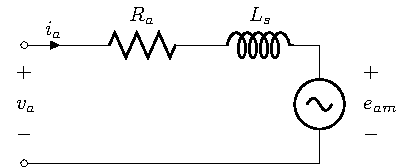
\includegraphics{figSynchronousMotorModel}
\begin{tikzpicture}
%grid
%\draw[gray,thick] (-2*\sRo,-2*\sRo) grid (2*\sRo,3*\sRo);
%\draw[gray,thin,xstep=0.1,ystep=0.1] (-2*\sRo,-2*\sRo) grid (2*\sRo,3*\sRo);
\draw (0,0) to [short,i={$i_a$},o-] ++(1,0) to [resistor,l={$R_a$}] ++(2,0) to [inductor,l={$L_s$}] ++(2,0) to [sinusoidal voltage source] ++(0,-2) to [short,-o](0,-2);
\draw node at (0,-1){$
\begin{aligned}
&+\\
&v_a\\
&-
\end{aligned} $};
%
\draw node at (6,-1){$
\begin{aligned}
&+\\
&e_{am}\\
&-
\end{aligned} $};
\end{tikzpicture}
\caption{معاصر موٹر کا مساوی دور یا ریاضی نمونہ۔}
\label{شکل_معاصر_موٹر_کا_مساوی_دور}
\end{figure}
اگر موٹر کی بجائے ایک معاصر جنریٹر کی بات ہوتی تب  جنریٹر برقی دباو پیدا کرتا اور برقی رو اس جنریٹر کے مثبت سر سے خارج ہوتا اور  ہمیں شکل \حوالہ{شکل_معاصر_موٹر_کا_مساوی_دور}  کی بجائے  شکل \حوالہ{شکل_معاصر_جنریٹر_کا_مساوی_دور}  حاصل ہوتا۔ شکل \حوالہ{شکل_معاصر_جنریٹر_کا_مساوی_دور} سے جنریٹر کی  مساوات لکھتے ہیں۔
\begin{figure}
\centering
%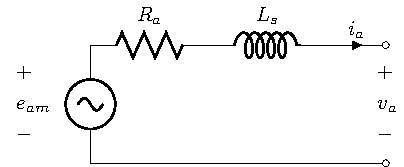
\includegraphics{figSynchronousGeneratorModel}
\begin{tikzpicture}
%grid
%\draw[gray,thick] (-2*\sRo,-2*\sRo) grid (2*\sRo,3*\sRo);
%\draw[gray,thin,xstep=0.1,ystep=0.1] (-2*\sRo,-2*\sRo) grid (2*\sRo,3*\sRo);
\draw (0,0) to [resistor,l={$R_a$}] ++(2,0) to [inductor,l={$L_s$}] ++(2,0) to [short,,i={$i_a$},-o] ++(1,0); 
\draw (5,-2) to [short,o-] (0,-2) to [sinusoidal voltage source] (0,0);

\draw node at (-1,-1){$
\begin{aligned}
&+\\
&e_{am}\\
&-
\end{aligned} $};
%
\draw node at (5,-1){$
\begin{aligned}
&+\\
&v_a\\
&-
\end{aligned} $};
\end{tikzpicture}
\caption{معاصر جنریٹر کا مساوی دور یا ریاضی نمونہ۔}
\label{شکل_معاصر_جنریٹر_کا_مساوی_دور}
\end{figure}

\begin{align}\label{مساوات_معاصر_جنریٹر_کی_مساوات}
e_{am}=i_a R_a+L_s \frac{\dif i_a}{\dif t}+v_a
\end{align}
دھیان رہے کہ جنریٹر کے مساوی دور میں برقی رو کا مثبت رخ، موٹر کے مساوی دور میں برقی رو کے مثبت رخ کا اُلٹ ہے۔مساوات \حوالہ{مساوات_معاصر_جنریٹر_کی_مساوات} کی  دوری سمتیہ\فرہنگ{دوری سمتیہ} روپ 
\begin{align}\label{مساوات_معاصر_جنریٹر_دوری_سمتیہ_مساوات}
\hat{E}_{am}= \hat{I}_a R_a+j \hat{I}_a X_s +\hat{V}_a
\end{align}
ہو گی جس کو شکل \حوالہ{شکل_معاصر_جنریٹر_کے_سادہ_مساوی_دور}-ا میں دکھایا گیا ہے۔
\begin{figure}
\centering
%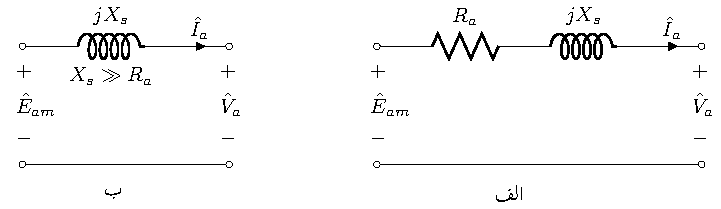
\includegraphics{figSynchronousGeneratorEquivalentCircuits}
\begin{subfigure}{0.55\textwidth}
\centering
\begin{tikzpicture}
\draw (0,0) to  [short,o-] (0.5,0) to[resistor,l={$R_a$}] ++(2,0) to [inductor,l={$j X_s$}] ++(2,0) to [short,,i={$\hat{I}_a$},-o] ++(1,0); 
\draw (5.5,-2) to [short,o-o] (0,-2);
\draw node at (0.2,-1){$
\begin{aligned}
&+\\
&\hat{E}_{am}\\
&-
\end{aligned} $};
%
\draw node at (5.5,-1){$
\begin{aligned}
&+\\
&\hat{V}_a\\
&-
\end{aligned} $};
\end{tikzpicture}%
\caption{}
\end{subfigure}\hfill
\begin{subfigure}{0.35\textwidth}
\centering
\begin{tikzpicture}
\draw (0,0) to  [short,o-] (0.5,0) to [inductor,l={$j X_s$}] ++(2,0) to [short,,i={$\hat{I}_a$},-o] ++(1,0); 
\draw (3.5,-2) to [short,o-o] (0,-2);
\draw node at (0.2,-1){$
\begin{aligned}
&+\\
&\hat{E}_{am}\\
&-
\end{aligned} $};
%
\draw node at (3.5,-1){$
\begin{aligned}
&+\\
&\hat{V}_a\\
&-
\end{aligned} $};
%text
\draw node at (1.5,-0.5) {$X_s \gg R_a$};
\end{tikzpicture}
\caption{}
\end{subfigure}%
\caption{معاصر جنریٹر کے مساوی ادوار۔}
\label{شکل_معاصر_جنریٹر_کے_سادہ_مساوی_دور}
\end{figure}

\ابتدا{مثال}
دو قطب، \عددیء{50} ہرٹز کا ایک معاصر جنریٹر \عددیء{40} ایمپیئر میدانی برقی رو پر  \عددیء{2100} وولٹ یک دوری موثر برقی دباو پیدا کرتا ہے۔اس مشین کے قوی اور میدانی لچھوں کا مشترکہ امالہ تلاش کریں۔

حل:\quad
	مساوات \حوالہ{مساوات_معاصر_موثر_پیدا_دباو}  سے  \عددی{L_{am}} حاصل کرتے ہیں۔
\begin{align}
L_{am}=\frac{\sqrt{2} E_{am}}{\omega I_m}=\frac{\sqrt{2}  \times 2100}{2 \times \pi \times 50 \times 40}=\SI{0.2363}{\henry}
\end{align}
\انتہا{مثال}
%
\حصہ{برقی طاقت کی منتقلی}
ٹرانسفارمر کا مساوی دور (ریاضی نمونہ) شکل \حوالہ{شکل_ٹرانسفارمر_سادہ_ماڈل}  میں  اور معاصر جنریٹر کا مساوی دور  شکل \حوالہ{شکل_معاصر_جنریٹر_کے_سادہ_مساوی_دور} میں دکھایا گیا ہے۔ یہ مساوی ادوار ایک دوسرے جیسے  ہیں، لہٰذا مندرجہ ذیل بیان دونوں کے لئے درست ہو گا، اگرچہ یہاں ہمیں صرف معاصر مشینوں سے دلچسپی ہے۔

معاصر مشینوں میں عموماً \عددیء{X_s} کی قیمت  \عددیء{R_a} کی قیمت سے  سو یا دو سو گنا زیادہ ہو گی۔ یوں \عددی{X_s>>R_a} ہو گا اور \عددی{R_a} کو رد کرنا ممکن ہو گا۔ اس طرح  شکل \حوالہ{شکل_معاصر_جنریٹر_کے_سادہ_مساوی_دور}-ا سے شکل \حوالہ{شکل_معاصر_جنریٹر_کے_سادہ_مساوی_دور}-ب حاصل ہو گا اور مساوات \حوالہ{مساوات_معاصر_جنریٹر_دوری_سمتیہ_مساوات} درج ذیل صورت اختیار کرے گی۔
\begin{align}\label{مساوات_معاصر_جنریٹر_دوری_سمتیہ_مساوات_سادہ}
\hat{E}_{am}= j \hat{I}_a X_s +\hat{V}_a
\end{align}

شکل \حوالہ{شکل_معاصر_جنریٹر_کے_سادہ_مساوی_دور}-ب کو  ایک لمحہ کے لئے ایک سادہ برقی دور تصور کریں جہاں  ایک متعاملہ \عددیء{j X_s}  کو بائیں  \عددیء{\hat{E}_{am}} اور دائیں  \عددیء{\hat{V}_a} برقی دباو فراہم کی گئی ہے۔ اس برقی دور میں برقی طاقت کی منتقلی پر غور کرتے ہیں۔

 شکل \حوالہ{شکل_معاصر_جنریٹر_کے_سادہ_مساوی_دور}-ب کی دوری سمتیہ صورت (مساوات \حوالہ{مساوات_معاصر_جنریٹر_دوری_سمتیہ_مساوات_سادہ}) کو  شکل \حوالہ{شکل_معاصر_جنریٹر_دوری_سمتیہ}  میں دکھایا گیا ہے۔شکل \حوالہ{شکل_معاصر_جنریٹر_دوری_سمتیہ}-ا میں  \عددیء{\hat{V}_a} کے لحاظ سے \عددیء{\hat{I}_a} زاویہ  \عددیء{\phi}  پیچھے  جبکہ شکل \حوالہ{شکل_معاصر_جنریٹر_دوری_سمتیہ}-ب میں  \عددیء{\phi}   آگے  ہے۔ زاویات افقی لکیر سے خلاف گھڑی ناپے جاتے ہیں لہٰذا شکل-ا میں \عددیء{\phi} منفی  اور \عددیء{\sigma} مثبت ہیں جبکہ شکل-ب میں دونوں زاویات مثبت ہیں۔
\begin{figure}
\centering
%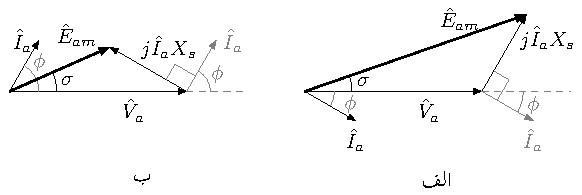
\includegraphics{figSynchronousGeneratorPhasorDiagram}
\begin{subfigure}{0.45\textwidth}
\centering
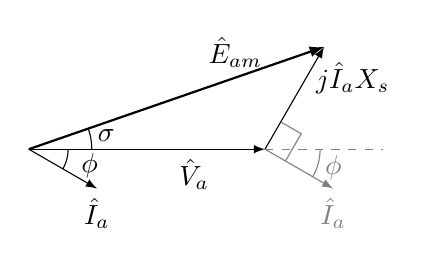
\begin{tikzpicture}
%grid
%\draw[gray,thick] (-2,-2) grid (5,2);
%\draw[gray,thin,xstep=0.1,ystep=0.1] (-2,-2) grid (5,2);
%
\draw[-latex](0,0)--(3,0)node[below,pos=0.7]{$\hat{V}_a$}coordinate(vEnd);
\draw[-latex](0,0)--++(-30:1)node[below]{$\hat{I}_a$};
\draw[] (0:0.5) arc (0:-30:0.5);
\draw[] (-15:0.8) node {$\phi$};
%
\draw[gray,-latex](vEnd)--++(-30:1)node[below]{$\hat{I}_a$};
\draw[-latex](vEnd)--++(60:1.5)coordinate(vTip)node[right,pos=0.7]{$j \hat{I}_a X_s$};
\draw[-latex,thick](0,0)--(vTip)node[above,pos=0.7]{$\hat{E}_{am}$};
\draw[gray] (vEnd)++(-30:0.3)--++(60:0.4)--++(150:0.3);
\draw[gray,dashed](vEnd)--++(0:1.5);
\draw[gray](vEnd)++(-30:0.7) arc (-30:0:0.7);
\draw[gray](vEnd)++(-15:0.9)node {$\phi$};
\draw (0.8,0) arc (0:19:0.8);
\draw (10:1) node{$\sigma$};
\end{tikzpicture}
\caption{}
\end{subfigure}\hfill
\begin{subfigure}{0.45\textwidth}
\centering
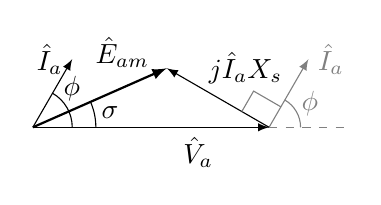
\begin{tikzpicture}
\draw[-latex](0,0)--(3,0)node[below,pos=0.7]{$\hat{V}_a$}coordinate(vEnd);
\draw[-latex](0,0)--++(60:1)node[left]{$\hat{I}_a$};
\draw[] (0:0.5) arc (0:60:0.5);
\draw[] (45:0.7) node {$\phi$};
\draw[gray,-latex](vEnd)--++(60:1)node[right]{$\hat{I}_a$};
\draw[-latex](vEnd)--++(150:1.5)coordinate(vTip)node[shift={(0:1)}]{$j \hat{I}_a X_s$};
\draw[-latex,thick](0,0)--(vTip)node[shift={(160:0.6)}]{$\hat{E}_{am}$};
\draw[gray] (vEnd)++(60:0.3)--++(150:0.4)--++(-120:0.3);
\draw[gray,dashed](vEnd)--++(0:1);
\draw[gray](vEnd)++(0:0.4) arc (0:60:0.4);
\draw[gray](vEnd)++(30:0.6)node {$\phi$};
\draw (0.8,0) arc (0:23:0.8);
\draw (11:1) node{$\sigma$};
\end{tikzpicture}
\caption{}
\end{subfigure}%
\caption{معاصر جنریٹر کا دوری سمتیہ۔}
\label{شکل_معاصر_جنریٹر_دوری_سمتیہ}
\end{figure}

 شکل \حوالہ{شکل_معاصر_جنریٹر_کے_سادہ_مساوی_دور}-ب میں طاقت \عددیء{p_v} بائیں سے دائیں منتقل ہو رہی ہے:
\begin{align}\label{مساوات_معاصر_طاقت_کی_منتقلی_الف}
p_v=V_a I_a \cos \phi
\end{align}
مساوات \حوالہ{مساوات_معاصر_جنریٹر_دوری_سمتیہ_مساوات_سادہ} اور شکل \حوالہ{شکل_معاصر_جنریٹر_دوری_سمتیہ}-ا  سے درج ذیل لکھا جا سکتا ہے۔
\begin{gather}
\begin{aligned}\label{مساوات_معاصر_رو_بالمقابل_دو_دباو}
\hat{I}_a=I_a \phase{\phi}&=\frac{\hat{E}_{am}-\hat{V}_a}{j X_s}\\
&=\frac{E_{am} \phase{\sigma} -V_a \phase {0}}{X_s \phase{\frac{\pi}{2}}}\\
&=\frac{E_{am}}{X_s} \phase{\sigma-\frac{\pi}{2}} -\frac{V_a}{X_s} \phase {-\frac{\pi}{2}}
\end{aligned}
\end{gather}
شکل \حوالہ{شکل_معاصر_جنریٹر_دوری_سمتیہ} سے واضح ہے کہ درج بالا مساوات میں \عددی{\hat{I}_a} کا حقیقی جزو  \عددیء{\hat{V}_a} کا ہم قدم ہو گا۔کسی بھی  دوری سمتیہ \عددی{K\phase{\alpha}} کو  حقیقی افقی جزو \عددی{K\cos\alpha} اور فرضی عمودی جزو \عددی{jK\sin\alpha} کا مجموعہ تصور کیا جا سکتا ہے۔ مساوات \حوالہ{مساوات_معاصر_رو_بالمقابل_دو_دباو} کے آخری قدم میں دائیں ہاتھ کے حقیقی اجزاء سے رو کا حقیقی جزو حاصل ہو گا :
\begin{gather}
\begin{aligned}
I_a \cos \phi&=\frac{E_{am}}{X_s} \cos \left(\sigma -\frac{\pi}{2} \right)-\frac{V_a}{X_s} \cos \left(-\frac{\pi}{2} \right)\\
&=\frac{E_{am}}{X_s} \sin \sigma
\end{aligned}
\end{gather}
اس کو مساوات \حوالہ{مساوات_معاصر_طاقت_کی_منتقلی_الف}  کے ساتھ ملا کر درج ذیل ملتا ہے۔
\begin{align}\label{مساوات_معاصر_سائن_خصوصیات}
p_v=\frac{V_a E_{am}}{X_s} \sin \sigma
\end{align}
تین دوری معاصر مشین کے لئے اس مساوات کو تین سے ضرب کرنا ہو گا:
\begin{align}\label{مساوات_معاصر_طاقت_بالمقابل_زاویہ}
p_v=\frac{3 V_a E_{am}}{X_s} \sin \sigma
\end{align}
مساوات \حوالہ{مساوات_معاصر_طاقت_بالمقابل_زاویہ} طاقت بالمقابل زاویہ\فرہنگ{طاقت بالمقابل زاویہ}\حاشیہب{power-angle law}\فرہنگ{power-angle law} کا قانون پیش کرتی ہے۔اٹل \عددیء{V_a} کی صورت میں جنریٹر \عددیء{E_{am}} یا (اور) \عددیء{\sigma} بڑھا کر طاقت بڑھا سکتا ہے۔گھومتے میدانی لچھے میں برقی رو بڑھا کر  \عددیء{E_{am}} بڑھایا جاتا ہے جو ایک حد تک کرنا ممکن ہو گا چونکہ میدانی  لچھے کی مزاحمت میں برقی توانائی ضائع ہونے سے لچھا گرم ہو گا جس کو خطرناک حد تک پہنچنے نہیں دیا جا سکتا ہے۔اسی طرح  \عددیء{\sigma} کو نوے زاویہ تک بڑھایا  جا سکتا ہے جس پر، کسی مخصوص \عددی{E_{am}} کے لئے، جنریٹر زیادہ سے زیادہ طاقت مہیا کرے گا:
\begin{align}\label{مساوات_معاصر_طاقت_انتہا}
p_{v,\textup{انتہا}}=\frac{3 V_a E_{am}}{X_s}&& (\sin 90^{\circ}=1)
\end{align}
حقیقت میں جنریٹر کی بناوٹ یوں کی جاتی ہے کہ  بناوٹی (قابل استعمال) طاقت نوے درجے سے کافی کم زاویہ پر ممکن ہو۔ نوے درجے پر جنریٹر کو قابو رکھنا مشکل ہوتا ہے۔
%
\begin{figure}
\centering
%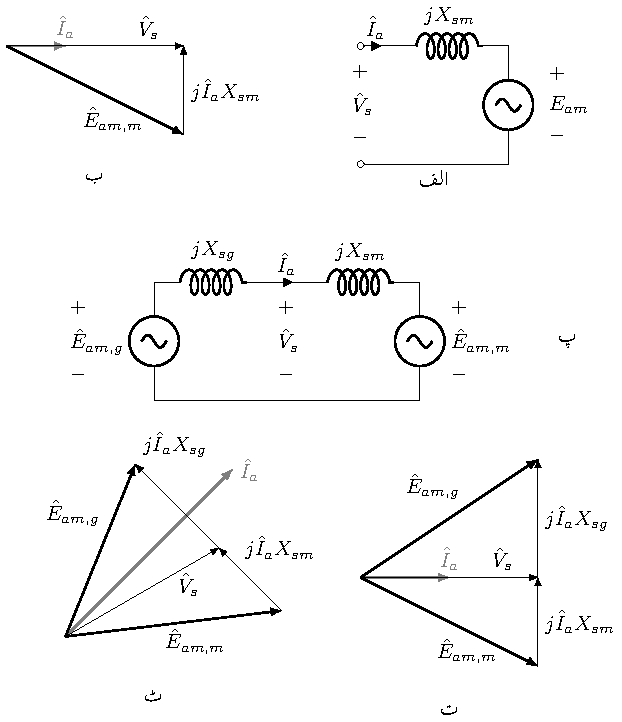
\includegraphics{figSynchronousGeneratorConnectedToMotor}
\begin{subfigure}{0.45\textwidth}
\centering
\begin{tikzpicture}
\draw(0,0) to [short,o-,i={$\hat{I}_a$}] ++(0.5,0) to [inductor,l={$j X_{sm}$}]++(2,0) to [sinusoidal voltage source] ++(0,-2) to [short,-o] (0,-2);
\draw node at (3.5,-1){$
\begin{aligned}
&+\\
&{E}_{am}\\
&-
\end{aligned}$};
\draw node at (0,-1){$\begin{aligned}
&+\\
&\hat{V}_a\\
&-
\end{aligned} $};
\end{tikzpicture}
\caption{}
\end{subfigure}\hfill
\begin{subfigure}{0.45\textwidth}
\centering
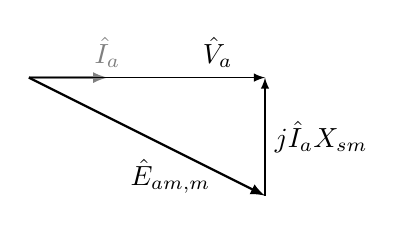
\begin{tikzpicture}
\draw[gray,thick,-latex](0,0)--++(0:1)node[above]{$\hat{I}_a$};
\draw[-latex](0,0)--++(0:3)node[above,pos=0.8]{$\hat{V}_a$}coordinate(vTip);
\draw[latex-](vTip)--++(-90:1.5)node[pos=0.5,right]{$j \hat{I}_aX_{sm}$}coordinate(ixStart);
\draw[-latex,thick](0,0)--(ixStart)node[below,pos=0.6]{$\hat{E}_{am,m}$};
\end{tikzpicture}
\caption{}
\end{subfigure}
\begin{subfigure}{1\textwidth}
\centering
\begin{tikzpicture}
\draw(0,0) to [sinusoidal voltage source] ++(0,2) to [inductor,l={$j X_{sg}$}]++(2,0) to [short,i={$\hat{I}_a$}] ++(0.5,0) to [inductor,l={$j X_{sm}$}] ++(2,0) to [sinusoidal voltage source]++(0,-2) to (0,0);
\draw node at (2.25,1){$\begin{aligned}
&+\\
&\hat{V}_a\\
&-
\end{aligned} $};
\draw node at (-1,1){$\begin{aligned}
&+\\
&\hat{E}_{am,g}\\
&-
\end{aligned} $};
\draw node at (5.5,1){$\begin{aligned}
&+\\
&\hat{E}_{am,m}\\
&-
\end{aligned} $};
\end{tikzpicture}
\caption{}
\end{subfigure}
\begin{subfigure}{0.45\textwidth}
\centering
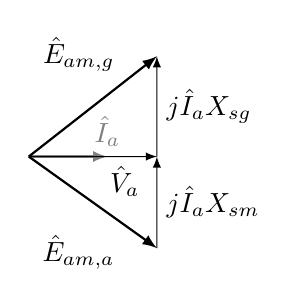
\begin{tikzpicture}
\pgfmathsetmacro{\Em}{2}
\pgfmathsetmacro{\Eg}{1686/1632*\Em}
\pgfmathsetmacro{\angM}{-35.548}
\pgfmathsetmacro{\angG}{38.047}
\draw[gray,thick,-latex](0,0)--++(0:1)node[above]{$\hat{I}_a$};
\draw[-latex,thick](0,0)--++(\angM:\Em)coordinate(kL)node[pos=0.75,below left]{$\hat{E}_{am,a}$};
\draw[-latex,thick](0,0)--++(\angG:\Eg)coordinate(kT)node[pos=0.75,above left]{$\hat{E}_{am,g}$};
\path(kL)--(kT)coordinate[pos=0.4773](kV)coordinate[pos=1](kE);
\draw[-latex](kL)--(kV)node[pos=0.5,right]{$j\hat{I}_aX_{sm}$};
\draw[-latex](kV)--(kE)node[pos=0.5,right]{$j\hat{I}_aX_{sg}$};
\draw[-latex](0,0)--(kV)node[pos=0.75,below]{$\hat{V}_a$};
\end{tikzpicture}
\caption{}
\end{subfigure}\hfill
\begin{subfigure}{0.45\textwidth}
\centering
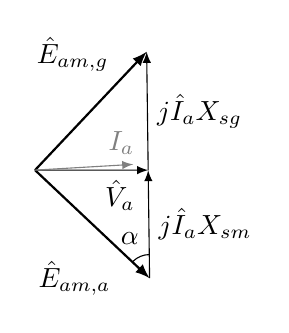
\begin{tikzpicture}
\pgfmathsetmacro{\Em}{2}
\pgfmathsetmacro{\Eg}{1686/1632*\Em}
\pgfmathsetmacro{\ang}{-43.327}
\pgfmathsetmacro{\angA}{90-43.327+\ang}
\draw[-latex,thick](0,0)--++(\ang:\Em)coordinate(kL)node[pos=0.75,below left]{$\hat{E}_{am,a}$};
\draw[-latex,thick](0,0)--++(90+\ang:\Eg)coordinate(kT)node[pos=0.75,above left]{$\hat{E}_{am,g}$};
\path(kL)--(kT)coordinate[pos=0.4773](kV)coordinate[pos=1](kE);
\draw[-latex](kL)--(kV)node[pos=0.5,right]{$j\hat{I}_aX_{sm}$};
\draw[-latex](kV)--(kE)node[pos=0.5,right]{$j\hat{I}_aX_{sg}$};
\draw[-latex](0,0)--(kV)node[pos=0.75,below]{$\hat{V}_a$};
\draw[-latex,gray](0,0)--++(\angA:1.25)node[above,xshift=-1ex]{$I_a$};
\draw(kL)++(0,0.3) arc (90:90+45:0.3);
\draw(kL)++(-0.25,0.5)node[]{$\alpha$};
\end{tikzpicture}
\caption{}
\end{subfigure}
\caption{معاصر جنریٹر معاصر موٹر چلا رہا ہے۔}
\label{شکل_معاصر_جنریٹر_موٹر_چلاتا_ہوا}
\end{figure}

\ابتدا{مثال}
ایک \عددیء{50} قطبی، ستارہ، تین دوری \عددیء{50} ہرٹز، \عددیء{2300} وولٹ دباو تار  پر چلنے والی \عددیء{1800} کلو وولٹ-ایمپیئر  معاصر مشین کا یک دوری  معاصر امالہ \عددیء{2.1} اوہم ہے۔
\begin{itemize}
\item
مشین کے برقی سروں پر \عددیء{2300} وولٹ دباو تار مہیا کیا جاتا ہے جبکہ اس کا میدانی برقی رو اتنا رکھا جاتا ہے کہ پورے بوجھ پر مشین کا جزو طاقت ایک کے برابر ہو۔ اس مشین سے زیادہ سے زیادہ کتنی قوت مروڑ حاصل کی جا سکتی ہے؟
\item
اس موٹر کو  \عددیء{2}  قطبی،  \عددیء{3000} چکر فی منٹ، تین دوری، ستارہ،  \عددیء{2300} وولٹ دباو تار پیدا کرنے والا \عددیء{2200}  کلو وولٹ-ایمپیئر کے معاصر جنریٹر سے چلایا جاتا ہے جس کا یک دوری معاصر امالہ \عددیء{2.3} اوہم ہے۔موٹر پر اس کا پورا برقی بوجھ لاد  کر جنریٹر کو معاصر رفتار پر چلاتے ہوئے دونوں مشینوں کے میدانی برقی رو تبدیل کیے جاتے ہیں حتیٰ کہ موٹر ایک جزو طاقت پر چلنے لگے۔دونوں مشینوں کا میدانی برقی رو یہاں برقرار رکھ کر موٹر پر بوجھ آہستہ آہستہ بڑھایا جاتا ہے۔اس صورت میں موٹر سے زیادہ سے زیادہ کتنی قوت مروڑ  حاصل کی جا سکتی ہے اور اس کی سروں پر دباو تار کتنا ہو گا؟ 
\end{itemize}

حل:
\begin{itemize}
\item
شکل \حوالہ{شکل_معاصر_جنریٹر_موٹر_چلاتا_ہوا}-ا اور \حوالہ{شکل_معاصر_جنریٹر_موٹر_چلاتا_ہوا}-ب سے رجوع کریں۔یک دوری برقی دباو اور کل برقی رو درج ذیل ہوں گے۔
\begin{align*}
\frac{2300}{\sqrt{3}}=\SI{1327.9}{\volt}\\
\frac{\num{1800000}}{\sqrt{3} \times 2300}=\SI{451.84}{\ampere}
\end{align*}
یوں درج ذیل ہو گا۔
\begin{align*}
\hat{E}_{am,m}&=\hat{V}_a-j \hat{I}_a X_{s,m}\\
&=1327.9 \phase {0\degree} -j 451.84 \phase {0\degree} \times 2.1\\
&=1327.9-j 948.864\\
&=1632 \phase{-35.548\degree}
\end{align*}
مساوات \حوالہ{مساوات_معاصر_طاقت_انتہا}  سے یک دوری زیادہ سے زیادہ برقی طاقت حاصل کرتے ہیں۔
\begin{align*}
p_{\textup{انتہا}}=\frac{1327.9 \times 1632}{2.1}=\SI{1031968}{\watt}
\end{align*}
اس طرح  تین دوری زیادہ سے زیادہ طاقت \عددیء{\num{3095904}} واٹ ہو گی۔\عددیء{50} ہرٹز اور \عددیء{50} قطب سے مشین کی معاصر میکانی رفتار مساوات \حوالہ{مساوات_گھومتے_مشین_برقی_میکانی_رفتار_تعلق}  کی مدد سے دو چکر فی سیکنڈ حاصل ہوتی ہے یعنی \عددیء{f_m=2}۔یوں مشین سے درج ذیل زیادہ سے زیادہ قوت مروڑ حاصل کی جا سکتی ہے۔
\begin{align*}
T_{\textup{انتہا}}=\frac{p_{\textup{انتہا}}}{2 \pi f_m}=\frac{3095904}{2 \times \pi \times 2}=\SI{246364}{\newton \meter}
\end{align*}
موٹر پر اس سے زیادہ قوت مروڑ کا بوجھ مسلط کرنے سے موٹر  رک جائے گی جبکہ جنریٹر کی رفتار بے قابو بڑھنے شروع ہو جائے گی۔ خود کار منقطع کار  اس لمحہ پر نظام کو روک دیگا۔
\item
شکل \حوالہ{شکل_معاصر_جنریٹر_موٹر_چلاتا_ہوا}-ج سے رجوع کریں۔اس مثال کے پہلے جزو کی طرح یہاں بھی موٹر کے برقی سروں پر دباو تار  \عددیء{2300} وولٹ اور  محرک برقی دباو \عددیء{1632} وولٹ ہوں گے۔ جنریٹر کا محرک برقی دباو درج ذیل ہو گا۔
\begin{align*}
\hat{E}_{am,g}&=\hat{V}_a+j  \hat{I}_a X_{s,g}\\
&=1327.9 \phase {0\degree} +j 451.84 \phase {0\degree} \times 2.3\\
&=1327.9+j 1039.233\\
&=1686 \phase{38.047\degree}
\end{align*}
یہ صورت شکل \حوالہ{شکل_معاصر_جنریٹر_موٹر_چلاتا_ہوا}-د میں دکھائی گئی ہے۔

جیسا شکل \حوالہ{شکل_معاصر_جنریٹر_موٹر_چلاتا_ہوا}-ھ میں دکھایا گیا ہے، موٹر اس  وقت زیادہ سے زیادہ طاقت پیدا کرے گی جب  \عددیء{\hat{E}_{am,g}} اور \عددیء{\hat{E}_{am,m}} آپس میں \عددیء{90\degree} زاویہ پر ہوں۔

یہاں  مساوات \حوالہ{مساوات_معاصر_طاقت_انتہا}  میں ایک معاصر امالہ کی بجائے موٹر اور جنریٹر کے  سلسلہ وار جڑے امالہ ہوں گے  اور دو برقی دباو اب موٹر اور جنریٹر کے محرک برقی دباو ہوں گے۔یوں موٹر کی یک دوری  زیادہ سے زیادہ طاقت درج ذیل ہو گی۔
\begin{align*}
p_{\textup{انتہا}}=\frac{1686 \times 1632}{2.3+2.1}=\SI{625352}{\watt}
\end{align*}	
اس طرح تین دوری طاقت  \عددیء{\num{1876056 }} واٹ  اور زیادہ سے زیادہ قوت مروڑ درج ذیل ہو گی۔
\begin{align*}
T_{\textup{انتہا}}=\frac{1876056}{2 \times \pi \times 2}=\SI{149291}{\newton \meter}
\end{align*}
\end{itemize}
شکل \حوالہ{شکل_معاصر_جنریٹر_موٹر_چلاتا_ہوا}-ھ میں \عددی{\hat{E}_{am,m}} اور \عددی{\hat{E}_{am,g}} آپس میں عمودی ہیں لہٰذا درج ذیل ہو گا۔
\begin{align*}
I_a(X_{s,g}+X_{s,m})&=\sqrt{E^2_{am,m}+E^2_{am,g}}=\SI{2346}{\volt}\\
I_a&=\frac{2346}{2.1+2.3}=\SI{533}{\ampere}\\
I_aX_{sg}&=533\times 2.1=\SI{1119.9}{\volt}\\
\alpha&=\tan^{-1}\frac{1686}{1632}=45.93^{\circ}
\end{align*} 
یوں دوری دباو \عددی{V_a}، جو صفر زاویہ پر تصور کیا جاتا ہے،  درج ذیل ہو گا۔
\begin{align*}
V_a=\sqrt{1632^2+1119.9^2-2\times 1632\times1119.9\times\cos 45.93^{\circ}}=\SI{1172.7}{\volt}
\end{align*}
لامتناہی نظام کی بجائے موٹر کو جنریٹر سے طاقت مہیا کر کے، موٹر پر بوجھ بڑھانے  سے موٹر کے سروں پر برقی دباو گھٹتا ہے جس کی بنا زیادہ سے زیادہ ممکنہ طاقت \عددی{\SI{3095}{\kilo\watt}} سے گھٹ کر \عددی{\SI{1876}{\kilo\watt}} رہ گئی ہے۔ موٹر کی سروں پر برقی دباو  \عددی{\hat{V}_a} اور برقی رو \عددی{\hat{I}_a} ہم قدم نہیں ہیں۔ 
\انتہا{مثال}
%
\حصہ{یکساں حال، برقرار چالو مشین کے خواص}
\جزوحصہ{معاصر جنریٹر: برقی بوجھ بالمقابل \عددیء{I_m} کے خط}
شکل \حوالہ{شکل_معاصر_جنریٹر_کے_سادہ_مساوی_دور}-ب کی دوری سمتیہ  مساوات
\begin{align}\label{مساوات_معاصر_دوری_جنریٹر_مساوات}
\hat{E}_{am}=\hat{V}_a+j \hat{I}_a X_s
\end{align}
میں \عددی{\hat{I}_a=I_a\phase{\phi}} لیتے ہوئے درج ذیل لکھا جا سکتا ہے
\begin{align}
E_{am}\phase{\sigma}=V_a \phase{0} +I_a X_s \phase{\frac{\pi}{2}+\phi}
\end{align}
جس کو بطور مخلوط عدد\فرہنگ{مخلوط عدد}\حاشیہب{complex number}
\begin{small}
\begin{align*}
E_{am} \cos \sigma +j E_{am} \sin \sigma&=V_a \cos 0+j V_a \sin 0 + I_a X_s \cos \left(\frac{\pi}{2}+\phi \right)+j I_a X_s \sin \left(\frac{\pi}{2}+\phi \right)\\
&=V_a  - I_a X_s \sin \phi+j I_a X_s \cos \phi\\
&=E_{am,x}+j E_{am,y}
\end{align*}
\end{small}
لکھ سکتے ہیں۔ اس  سے \عددیء{\abs{\hat{E}_{am}}} یعنی  \عددیء{E_{am}}  حاصل کرتے ہیں۔
\begin{gather}
\begin{aligned}\label{مساوات_معاصر_رو_بالمقابل_دباو}
\abs{\hat{E}_{am}}=E_{am}&=\sqrt{E_{am,x}^2+E_{am,y}^2}\\
&=\sqrt{(V_a  - I_a X_s \sin \phi)^2+(I_a X_s \cos \phi)^2}\\
&=\sqrt{V_a^2+\left(I_a X_s\right)^2 -2 V_a I_a X_s \sin \phi}
\end{aligned}
\end{gather}
جنریٹر کے سروں پر  \عددیء{V_a} اٹل رکھتے ہوئے مختلف \عددیء{\phi} کے لئے \عددیء{E_{am}} بالمقابل \عددیء{I_a} کے خط شکل \حوالہ{شکل_معاصر_بار_بالمقابل_میدانی_رو}  میں دکھائے گئے ہیں۔یہ خطوط مساوات \حوالہ{مساوات_معاصر_رو_بالمقابل_دباو} دیتی ہے۔ چونکہ \عددیء{E_{am}}  اور  \عددیء{I_m}  راست متناسب ہیں اور کسی  مخصوص جزو طاقت اور معین \عددیء{V_a} کے لئے جنریٹر کی طاقت \عددیء{I_a} کے   راست متناسب ہوتی ہے لہٰذا یہی ترسیمات \عددیء{I_m} بالمقابل جنریٹر کی طاقت کو بھی ظاہر کرتی ہیں۔
\begin{figure}
\centering
%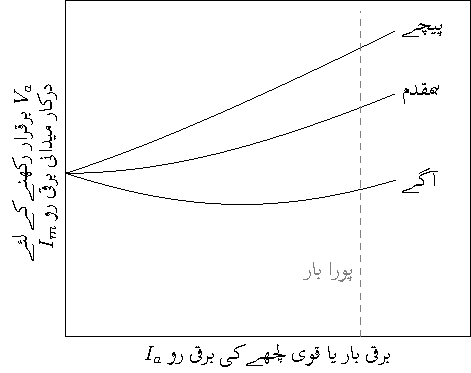
\includegraphics{figSynchronousCompoundingCurves}
\begin{tikzpicture}
\begin{axis}[
	ticks=none,
	xmin=0,
	xmax=1.35,
	ymin=0,
%	axis lines=middle,
%	axis y line=middle,
	axis line style=-,
%	ytick={0.25,0.5},
%	yticklabels={50,100},
%	xtick style={draw=none},
	ylabel style={align=right},
	ylabel={\RL{ $V_a$ برقرار رکھنے کے لئے} \\ \RL{ درکار میدانی برقی رو $I_m$}},
	xlabel style={align=right},
	xlabel={\RL{برقی بار یا قوی لچھے کا برقی رو $I_a$}},
]
\newcommand\tka{0}
\addplot[
black,
domain=0:1.1,
samples=100,
]
{sqrt(1+x*x-2*x*sin(\tka))} node[right] {\RL{ہم قدم}} ;
%==
\newcommand\tkb{-36}
\addplot[
black,
domain=0:1.1,
samples=100,
]
{sqrt(1+x*x-2*x*sin(\tkb))} node[right] {تاخیری} ;
%=====
\newcommand\tkc{36}
\addplot[
black,
domain=0:1.1,
samples=100,
]
{sqrt(1+x*x-2*x*sin(\tkc))} node[right] {پیش قدم} ;
\addplot[dashed]coordinates {(1,0)(1,2)}node[pos=0.2,left]{\RL{پورا بوجھ}};
\end{axis}
\end{tikzpicture}
\caption{جنریٹر: برقی بوجھ بالمقابل \عددیء{I_m} کے خط}
\label{شکل_معاصر_بار_بالمقابل_میدانی_رو}
\end{figure}
\جزوحصہ{معاصر موٹر:\عددیء{I_a}   بالمقابل \عددیء{I_m}  کے خط}
معاصر موٹر کا مساوی دور (ریاضی نمونہ) شکل \حوالہ{شکل_معاصر_موٹر_کا_مساوی_دور}   اور دوری سمتیہ شکل  \حوالہ{شکل_معاصر_موٹر_کی_دوری_سمتیہ} میں دکھایا گیا ہے۔  مزاحمت نظرانداز کر کے اس کی مساوات لکھتے ہیں۔
\begin{gather}
\begin{aligned}
\hat{V}_a&=\hat{E}_{am}+j \hat{I}_a X_s\\
V_a \phase{0}&=E_{am} \phase{\sigma} +j I_a \phase{\phi} X_s\\
&=E_{am} \phase{\sigma} +I_a X_s \phase{\frac{\pi}{2}+\phi}
\end{aligned}
\end{gather}
اس مساوات میں موٹر پر لاگو برقی دباو \عددیء{\hat{V}_a} کے حوالہ سے زاویات کی پیمائش کی گئی ہے لہٰذا  \عددیء{\hat{V}_a}  کا زاویہ صفر ہو گا۔یاد رہے کہ مثبت زاویہ کی پیمائش افقی لکیر سے گھڑی کے مخالف رخ ہو گی  لہٰذا \اصطلاح{پیش} زاویہ\حاشیہب{leading angle} مثبت اور \اصطلاح{تاخیری} زاویہ\حاشیہب{lagging angle} منفی ہو گا۔ اس مساوات سے امالی دباو \عددیء{E_{am}}  حاصل کرتے ہیں۔
\begin{align*}
E_{am}\phase{\sigma}&=V_a \phase{0}-I_a X_s \phase{\frac{\pi}{2}+\phi}\\
&=V_a -I_a X_s  \cos \left( \frac{\pi}{2}+\phi\right)- j I_a X_s \sin \left(\frac{\pi}{2}+\phi \right)\\
&=V_a +I_a X_s \sin \phi-j I_a X_s \cos \phi
\end{align*}
یوں \عددی{\abs{E_{am}}} درج ذیل ہو گا۔
\begin{gather}
\begin{aligned}\label{مسوات_معاصر_دوری_مساوات}
\abs{E_{am}}&=\sqrt{\left(V_a +I_a X_s \sin \phi \right)^2+\left(I_a X_s \cos \phi \right)^2}\\
&=\sqrt{V_a^2+I_a^2 X_s^2+ 2 V_a I_a X_s \sin \phi}
\end{aligned}
\end{gather}
موٹر پر لاگو برقی دباو اور اس پر میکانی بوجھ کو \عددیء{\SI{0}{\percent}}، \عددیء{\SI{25}{\percent}} اور \عددیء{\SI{75}{\percent}} پر رکھ کر، موٹر کے \عددیء{E_{am}} بالمقابل  \عددیء{I_a} خطوط،  مساوات \حوالہ{مسوات_معاصر_دوری_مساوات} سے  شکل \حوالہ{شکل_معاصر_برقی_رو_بالمقابل_برقی_دباو}   میں  ترسیم کیے گئے ہیں۔ چونکہ امالی دباو \عددیء{I_m} کا راست متناسب ہوتا ہے  لہٰذا یہی موٹر کے \عددیء{I_m} بالمقابل \عددیء{I_a} خطوط بھی ہوں گے۔ان میں سے ہر خط ایک معین میکانی بوجھ \عددیء{p} کے لئے ہے جہاں \عددی{p} درج ذیل ہو گا۔
\begin{align}\label{مساوات_معاصر_طاقت_برابر_دباو_رو_جزو_طاقت}
p=V_a I_a \cos \phi
\end{align}
%
\begin{figure}
\centering
%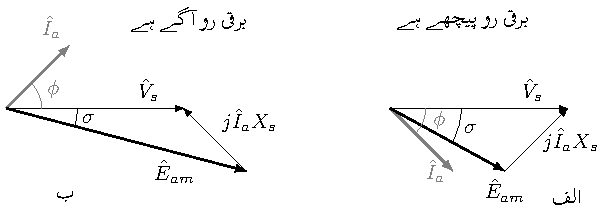
\includegraphics{figSynchronousMotorPhasorDiagram}
\begin{subfigure}{0.40\textwidth}
\centering
\begin{tikzpicture}
\pgfmathsetmacro{\phaseI}{-45}
\pgfmathsetmacro{\phaseV}{0}
\draw[thick,-latex](0,0)--++(\phaseI:1.5)node[left]{$\hat{I}_a$};
\draw[-latex](0,0)--++(\phaseV:3)node[above,pos=0.8]{$\hat{V}_{s}$}coordinate(vTip);
\draw[latex-](vTip)--++(-90+\phaseI:1.5)node[pos=0.5,right]{$j \hat{I}_aX_{s}$}coordinate(ixStart);
\draw[-latex,thick](0,0)--(ixStart)node[below]{$\hat{E}_{am}$};
%text
\draw[](0:0.6) arc (0:\phaseI:0.6);
\draw[](-13:0.85)node{$\phi$};
%
\draw(0:1.2) arc (0:-28:1.2);
\draw(-14:1.4)node{$\sigma$};
\draw node[right] at (0,1.5){\RL{برقی رو تاخیری ہے}};
\end{tikzpicture}
\caption{}
\end{subfigure}\hfill
\begin{subfigure}{0.50\textwidth}
\centering
\begin{tikzpicture}
\pgfmathsetmacro{\phaseI}{45}
\pgfmathsetmacro{\phaseV}{0}
\draw[thick,-latex](0,0)--++(\phaseI:1.5)node[above left]{$\hat{I}_a$};
\draw[-latex](0,0)--++(\phaseV:3)node[above,pos=0.8]{$\hat{V}_{s}$}coordinate(vTip);
\draw[latex-](vTip)--++(-90+\phaseI:1.5)node[pos=0.5,above right]{$j \hat{I}_aX_{s}$}coordinate(ixStart);
\draw[-latex,thick](0,0)--(ixStart)node[below,pos=0.7]{$\hat{E}_{am}$};
%text
\draw[](0:0.6) arc (0:\phaseI:0.6);
\draw[](22.5:0.85)node{$\phi$};
%
\draw(0:1.2) arc (0:-14:1.2);
\draw(-7:1.4)node{$\sigma$};
\draw node[right] at (2,1.5){\RL{برقی رو پیش قدم ہے}};
\end{tikzpicture}
\caption{}
\end{subfigure}%
\caption{موٹر کا دوری سمتیہ۔}
\label{شکل_معاصر_موٹر_کی_دوری_سمتیہ}
\end{figure}
%
\begin{figure}
\centering
%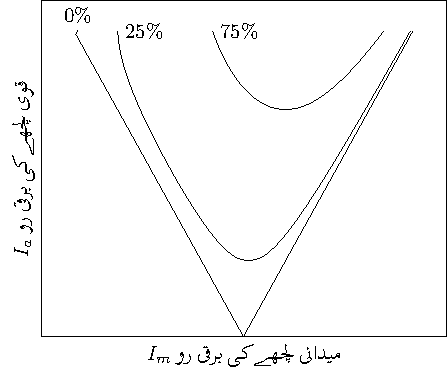
\includegraphics{figSynchronousVcurves}
\begin{tikzpicture}
\begin{axis}[
	ticks=none,
%	xmin=0,
%	xmax=1.35,
	ymin=0,
%	axis lines=middle,
%	axis y line=middle,
	axis line style=-,
%	ytick={0.25,0.5},
%	yticklabels={50,100},
%	xtick style={draw=none},
	ylabel style={align=right},
	ylabel={\RL{قوی لچھے کا برقی رو $I_a$}},
	xlabel style={align=right},
	xlabel={\RL{میدانی لچھے کا برقی رو $I_m$}},
]
%
\def\p{0}
\addplot[black,domain=\p*100:101,samples=100,]({sqrt(1+x/100*x/100-2*sqrt(x/100*x/100-\p*\p))},{x}) node [above,xshift=-1ex]{$\SI{0}{\percent}$} ;
\addplot[black,domain=\p*100:101,samples=100,]({sqrt(1+x/100*x/100+2*sqrt(x/100*x/100-\p*\p))},{x}) ;   %}
%
\def\p{0.25}
\addplot[black,domain=\p*100:101,samples=100,]({sqrt(1+x/100*x/100-2*sqrt(x/100*x/100-\p*\p))},{x}) node [above]{$\SI{25}{\percent}$} ;
\addplot[black,domain=\p*100:101,samples=100,]({sqrt(1+x/100*x/100+2*sqrt(x/100*x/100-\p*\p))},{x}) ; 
%
\def\p{0.75}
\addplot[black,domain=\p*100:101,samples=100,]({sqrt(1+x/100*x/100-2*sqrt(x/100*x/100-\p*\p))},{x}) node [above]{$\SI{75}{\percent}$} ;
\addplot[black,domain=\p*100:101,samples=100,]({sqrt(1+x/100*x/100+2*sqrt(x/100*x/100-\p*\p))},{x}) ; 
\end{axis}
\draw[dashed] (3.41,0) to [out=100,in=-100] node[pos=0.65,sloped,above,font=\small]{\RL{جزو طاقت \عددی{0.8} تاخیری}}
(3.41,5);
\draw[dashed] (3.41,0) to [out=90,in=-110] node[pos=0.60,sloped,above,font=\small]{\RL{جزو طاقت  \عددی{1}ہم قدم}}
(4.5,5);
\draw[dashed] (3.41,0) to [out=80,in=-120] node[pos=0.70,sloped,below,font=\small]{\RL{جزو طاقت \عددی{0.8} پیش قدم}}
(5.5,5);
\end{tikzpicture}
\caption{موٹر کی $I_{m}$ بالمقابل $I_a$ ترسیم۔}
\label{شکل_معاصر_برقی_رو_بالمقابل_برقی_دباو}
\end{figure}

اس مساوات کے تحت  \عددیء{p} اور \عددیء{V_a} تبدیل کیے بغیر  جزو طاقت تبدیل کر کے \عددیء{I_a} تبدیل کیا جا سکتا ہے۔ شکل \حوالہ{شکل_معاصر_برقی_رو_بالمقابل_برقی_دباو} کے حصول میں  مساوت \حوالہ{مسوات_معاصر_دوری_مساوات}  کو مساوات \حوالہ{مساوات_معاصر_طاقت_برابر_دباو_رو_جزو_طاقت}  کی مدد سے ترسیم کیا جاتا ہے۔مخصوص \عددیء{V_a} اور \عددیء{p} کے لئے مختلف \عددیء{I_a} پر مساوات \حوالہ{مساوات_معاصر_طاقت_برابر_دباو_رو_جزو_طاقت}   سے \عددیء{\phi} حاصل کیا جاتا ہے۔اس کے بعد  ہر انفرادی \عددیء{I_a} اور  مطابقتی  \عددیء{\phi}  کو مساوات  \حوالہ{مسوات_معاصر_دوری_مساوات} میں پر  کر کے \عددیء{E_{am}} حاصل کیا جاتا ہے۔ مخصوص \عددی{p} کے لئے   \عددیء{E_{am}} بالمقابل \عددیء{I_a} ترسیم کیے جاتے ہیں۔ شکل \حوالہ{شکل_معاصر_برقی_رو_بالمقابل_برقی_دباو} میں \عددی{\SI{0}{\percent}}، \عددی{\SI{25}{\percent}} اور \عددی{\SI{75}{\percent}} طاقت کے لئے ترسیمات پیش کی گئی ہیں۔

موٹر کے خطوط سے واضح ہے کہ \عددیء{I_m}  تبدیل کر کے موٹر کا جزو طاقت تبدیل کیا جا سکتا ہے۔ یوں موٹر کو \اصطلاح{پیش} زاویہ یا \اصطلاح{تاخیری} زاویہ  پر چلایا جا سکتا ہے۔ موٹر کو پیش زاویہ چلا کر بطور ایک \اصطلاح{برق گھیر}\فرہنگ{برق گھیر}\حاشیہب{capacitor}\فرہنگ{capacitor}  استعمال کیا جا  سکتا ہے۔ حقیقت میں ایسا نہیں کیا جاتا ہے چونکہ معاصر موٹر سے برق گھیر زیادہ سستا دستیاب ہوتا ہے۔ 

\حصہ{کھلا دور  اور کسر دور  معائنہ}
معاصر مشین کا مساوی دور بنانے کے لئے مساوی دور کے اجزاء جاننا لازم ہے جنہیں دو قسم کے معائنوں سے معلوم کیا جاتا ہے۔ انہیں کھلا دور معائنہ اور کسر دور معائنہ کہتے ہیں۔ان معائنوں سے قالب کے سیرابیت کے اثرات بھی اجاگر ہوتے ہیں۔اسی قسم کے معائنے ٹرانسفارمر کے  بھی کیے جاتے ہیں جہاں  کھلا دور معائنہ ٹرانسفارمر کے بناوٹی  برقی دباو جبکہ کسر دور معائنہ بناوٹی  برقی رو پر کیا جاتا ہے۔یہاں بھی ایسا کیا جائے گا۔ 

\جزوحصہ{کھلا دور معائنہ}
معاصر مشین کے برقی سرے کھلا رکھ کر، مشین کو معاصر رفتار پر گھماتے ہوئے مختلف \عددیء{I_m} پر پیدا برقی دباو \عددیء{V_a}  مشین کے سروں پر  ناپا جاتا ہے ۔شکل \حوالہ{شکل_معاصر_کھلے_دور_خط}-ا میں پیمائشی  رو \عددی{I_m} بالمقابل دباو \عددی{V_a}  کی  ترسیم  دکھائی گئی ہے۔ یہ ترسیم مشین کی کھلا دور خاصیت ظاہر کرتی ہے۔ یہ ترسیم مشین بنانے والے بھی مہیا کر سکتے ہیں۔

اس کتاب کے حصہ \حوالہ{حصہ_مقناطیسی_دور_مقناطیسی_مادہ_کے_خصوصیات} میں بتایا گیا  کہ قالب پر لاگو مقناطیسی دباو بڑھانے سے قالب میں مقناطیسی بہاو بڑھتا ہے البتہ جلد ہی قالب سیراب ہو جاتا ہے۔یہ اثر  شکل \حوالہ{شکل_معاصر_کھلے_دور_خط}-ا میں ترسیم کے جھکاو  سے واضح ہے۔قالب سیراب نہ ہونے کی صورت میں  ترسیم  نقطہ دار سیدھی لکیر کی پیروی کرتی۔مشین کا بناوٹی برقی دباو اور اس کے حصول کے لئے درکار  رو \عددیء{I_{m0}} بھی دکھائے گئے ہیں۔
\begin{figure}
\centering
%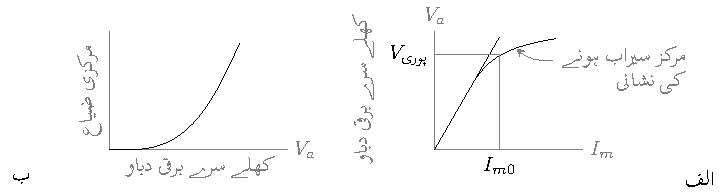
\includegraphics{figSynchronousOpenCircuitCharacteristic}
\begin{subfigure}{0.45\textwidth}
\centering
\begin{tikzpicture}
%axis
\draw[] (0,0)--(2.5,0)node[right]{$I_m$};
\draw[] (0,0)--(0,2)node[above]{$V_{a}$};
%curves
\draw[thick,dashed] (60:1.3)--(60:2.2);
\draw[thick,name path=kCur](0,0)--++(60:1.3) to [out=60,in=190] ++(1.4,0.75)coordinate(ktext);
\draw(ktext)node[below right,align=right]{\RL{ترسیم کا جھکاو، قالب}\\
 \RL{کی سیرابیت کی بنا ہے}};
\draw[] (1.4,1.7)++(0.025,-0.025) to [out=-45,in=180] (2,1.5);
\draw node[rotate=90] at (-0.4,0.65){\RL{\small{کھلا دور برقی دباو}}};
%
\path[name path=kVert](1.25,0)--++(0,2);
\draw[name intersections={of={kVert and kCur}}](1.25,0)node[below]{$I_{m0}$}--(intersection-1)--++(-1.25,0)node[left,yshift=0.5ex]{$V_{\textup{بناوٹی}}$};
\end{tikzpicture}
\caption{}
\end{subfigure}\hfill
\begin{subfigure}{0.45\textwidth}
\centering
\begin{tikzpicture}
%axis
\draw[] (0,0)--(3,0)node[right]{$V_a$};
\draw[] node at (1.5,-0.3){\RL{کھلا دور برقی دباو}};
\draw[] (0,0)--(0,2)node[xshift=-0.35cm,rotate=90,pos=0.5]{\RL{قالبی ضیاع}};
%curves
\draw[thick] (0,0)--++(0.4,0) to [out=0,in=-115] (2.2,1.8);
\end{tikzpicture}%
\caption{}
\end{subfigure}%
\caption{کھلا دور خط اور قالبی ضیاع۔}
\label{شکل_معاصر_کھلے_دور_خط}
\end{figure}

کھلا دور معائنہ کے دوران دھرے پر  میکانی طاقت \عددیء{p_1} کی پیمائش بے بوجھ مشین کا ضیاع طاقت  دے گی۔ اس کا بیشتر حصہ رگڑی ضیاع، کچھ قالبی ضیاع  اور کچھ گھومتے لچھے کا ضیاع  ہو گا۔یاد رہے  گھومتے لچھے کو عموماً دھرے پر نسب یک سمت  جنریٹر برقی توانائی فراہم کرتا ہے جس کو از خود  طاقت محرک\حاشیہد{گھومتے لچھے کو توانائی یک سمت رو  جنریٹر مہیا کرتا ہے اور اس جنریٹر کو دھرے سے توانائی موصول ہوتی ہے۔} فراہم کرتا ہے۔رگڑی ضیاع کا مشین پر لدے بوجھ سے کوئی خاص تعلق نہیں پایا جاتا ہے لہٰذا  بے بوجھ مشین اور بوجھ بردار مشین  کا رگڑی ضیاع ایک جیسا تصور کیا جاتا ہے۔

رو \عددیء{I_m}  صفر رکھتے ہوئے دوبارہ دھرے پر میکانی طاقت \عددیء{p_2} کی پیمائش صرف رگڑی ضیاع دے گا۔ان پیمائشوں کا فرق  \عددیء{(p_1-p_2)} قالبی ضیاع  اور گھومتے لچھے کا برقی ضیاع  ہو گا۔گھومتے لچھے میں برقی ضیاع بہت کم ہوتا ہے اور اس کو عموماً قالب کے ضیاع کا حصہ تصور کیا جاتا ہے۔ یوں  پیمائش کردہ قالبی ضیاع کی ترسیم شکل  \حوالہ{شکل_معاصر_کھلے_دور_خط}-ب میں دی گئی ہے۔

\جزوحصہ{کسر دور معائنہ}
معاصر مشین کو معاصر رفتار پر بطور جنریٹر  چلاتے ہوئے  ساکن لچھا کسر دور کر کے مختلف \عددیء{I_m} پر کسر دور برقی رو \عددیء{I_a} ناپا جاتا ہے۔ ان کی ترسیم شکل \حوالہ{شکل_معاصر_کسر_دور_اور_کھلے_دور_خط}-ا میں دی گئی ہے جو کسر دور مشین کی خاصیت ظاہر کرتی ہے۔ 

 کسر دور معائنہ کے دوران  دھیان رہے  کہ \عددیء{I_a}  خطرناک حد تک  بڑھ نہ جائے۔  جنریٹر کے بناوٹی \عددیء{I_{a}}  یا اس سے دگنی قیمت  سے رو کو  کم رکھا جاتا ہے۔ایسا نہ کرنے سے مشین گرم ہو کر تباہ ہو سکتی ہے۔

کسر دور مشین میں بناوٹی برقی دباو کے دس سے پندرہ فی صد برقی دباو پر مشین میں سو فی صد برقی رو پایا جاتا ہے۔ اتنا کم برقی دباو حاصل کرنے کے لئے خلائی درز میں اسی تناسب سے  کم مقناطیسی بہاو درکار ہو گا۔ 
\begin{figure}
\centering
%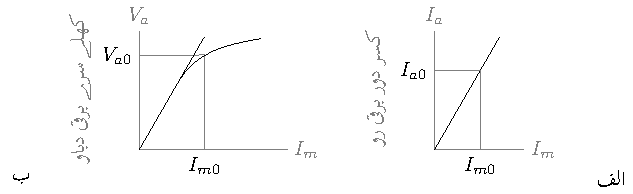
\includegraphics{figSynchronousShortCircuitCharacteristic}
\begin{subfigure}{0.45\textwidth}
\centering
\begin{tikzpicture}
\pgfmathsetmacro{\kIa}{1.25*tan(50)}
%axis
\draw[] (0,0)--(1.75,0)node[right]{$I_m$};
\draw[] (0,0)--(0,2)node[above]{$I_{a }$};
\draw[] node[rotate=90] at (-1,1){\RL{کسر دور برقی رو}};
%curves
\draw[thick] (0,0)--++(50:2.5);
%
\draw[](1.25,0)node[below]{$I_{m0}$}--(1.25,\kIa)--(0,\kIa)node[left]{$I_{a0}$};
\end{tikzpicture}%
\caption{}
\end{subfigure}\hfill
\begin{subfigure}{0.45\textwidth}
\centering
\begin{tikzpicture}
\draw[] node[rotate=90] at (-1,1){\RL{کھلا دور برقی دباو}};
%axis
\draw[] (0,0)--(2.5,0)node[right]{$I_m$};
\draw[name path=kYaxis] (0,0)--(0,2)node[above]{$V_a$};
%curves
\draw[thick] (0,0)--++(60:1.3);
\draw[thick,dashed] (0,0)++(60:1.3)--(60:2.2);
\draw[thick,name path=kCur](0,0)++(60:1.3) to [out=60,in=190] ++(1.4,0.75);
%
\path[name path=kVert](1.25,0)--++(0,2);
\draw[name intersections={of={kVert and kCur}}](1.25,0)node[below]{$I_{m0}$}--(intersection-1)--++(-1.25,0)node[left]{$V_{a0}$};
\end{tikzpicture}
\caption{}
\end{subfigure}%
\caption{کسر دور خط اور کھلے دور خط۔}
\label{شکل_معاصر_کسر_دور_اور_کھلے_دور_خط}
\end{figure}

شکل \حوالہ{شکل_معاصر_جنریٹر_کے_سادہ_مساوی_دور}-ا  میں جنریٹر کا مساوی برقی دور دکھایا گیا ہے جسے  شکل \حوالہ{شکل_معاصر_امالہ_معاصر}  میں کسر دور دکھایا گیا ہے۔یوں درج ذیل ہو گا۔
\begin{align}
\hat{E}_{am}=\hat{I}_a R_a+j \hat{I}_a X_s
\end{align}
\عددی{X_s>>R_a} کی بنا مزاحمت \عددیء{R_a}  نظر انداز کر کے اس مساوات سے معاصر امالہ حاصل ہو گا۔
\begin{align}\label{مساوات_معاصر_معاصر_امالہ_پیمائش}
X_s=\frac{\abs{\hat{E}_{am}}}{\abs{\hat{I}_a}}=\frac{E_{am}}{I_a}
\end{align}
%
\begin{figure}
\centering
%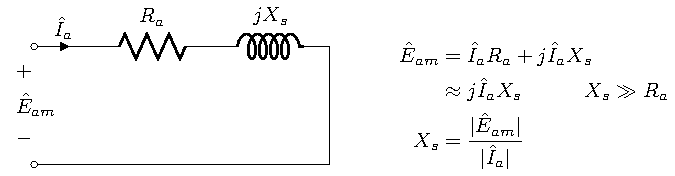
\includegraphics{figSynchronousReactanceSynchronous}
\begin{tikzpicture}
 \draw(0,0) to [short,o-,i={$\hat{I}_a$}] ++(1,0) to [resistor,l={$R_a$}] ++(2,0) to [inductor,l={$j X_s$}] ++(2,0) to ++(0,-2) to [short,-o] (0,-2);
\draw node at (0,-1){$
\begin{aligned}
&+\\
&\hat{E}_{am}\\
&-
\end{aligned} $};
%txt
\draw node[right] at (6,-1){$
\begin{aligned}
\hat{E}_{am}&=\hat{I}_a R_a +j \hat{I}_a X_s\\
&\approx j \hat{I}_a X_s \quad \quad \quad X_s \gg R_a\\
X_s&=\frac{|\hat{E}_{am}|}{|\hat{I}_a|}
\end{aligned}
$};
\end{tikzpicture}
\caption{معاصر امالہ۔}
\label{شکل_معاصر_امالہ_معاصر}
\end{figure}
مساوات \حوالہ{مساوات_معاصر_معاصر_امالہ_پیمائش} میں \عددیء{\hat{I}_a} کسر دور مشین کا برقی رو اور \عددیء{\hat{E}_{am}}  اسی حال میں مشین کے ایک دور کا امالی دباو ہے۔ کھلے دور مشین میں \عددیء{\hat{I}_a} صفر ہوتا ہے ۔مساوات \حوالہ{مساوات_معاصر_دوری_جنریٹر_مساوات} سے واضح ہے کہ  \عددیء{\hat{I}_a} صفر ہونے کی صورت میں \عددیء{\hat{E}_{am}}  اور \عددیء{\hat{V}_a} برابر ہوں گے۔ یوں  کسی معین \عددیء{I_{m0}} پر شکل \حوالہ{شکل_معاصر_کسر_دور_اور_کھلے_دور_خط}-ا سے  \عددیء{I_{a0}} اور شکل \حوالہ{شکل_معاصر_کسر_دور_اور_کھلے_دور_خط}-ب سے \عددیء{V_{a0}} پڑھ کر \عددیء{X_s} کی قیمت حاصل کی جا سکتی ہے۔
\begin{align}\label{مساوات_معاصر_امالہ_پیمائش}
X_s=\frac{V_{a0}}{I_{a0}}
\end{align}
معاصر امالہ کو عموماً مشین کے پورے (بناوٹی) برقی دباو پر معلوم کیا جاتا ہے تا کہ قالب کی سیرابیت کے اثرات کو بھی شامل ہوں۔

مشین کو ستارہ نما تصور کر کے اس کا یک دوری \عددیء{X_s} حاصل کیا جاتا ہے۔یوں اگر معائنہ میں مشین کا تار برقی دباو\حاشیہب{line voltage} ناپا گیا ہو تب ضروری ہے کہ اس  کو \عددیء{\sqrt{3}} سے تقسیم کر کے  یک دوری  دباو حاصل کر کے مساوات
 \حوالہ{مساوات_معاصر_امالہ_پیمائش} میں استعمال کیا جائے۔
\begin{align}
V_{\textup{یکدوری}}=\frac{V_{\textup{تار}}}{\sqrt{3}}
\end{align}
%
\ابتدا{مثال}
ایک  \عددیء{75}  کلو وولٹ-ایمپیئر، ستارہ،  \عددیء{415} وولٹ پر چلنے والی تین دوری معاصر مشین کا کھلا دور اور کسر دور معائنہ کیا گیا۔حاصل نتائج درج ذیل ہیں۔
\begin{itemize}
\item
کھلا دور معائنہ:\عددیء{V_{\textup{تار}}=\SI{415}{\volt}} اور \عددیء{I_m=\SI{3.2}{\ampere}} ہیں۔
\item
کسر دور معائنہ:
جس لمحہ قوی لچھے کا برقی رو \عددیء{\SI{104}{\ampere}} تھا اس لمحہ میدانی لچھے کا برقی رو \عددیء{\SI{2.48}{\ampere}} تھا اور جس لمحہ  قوی لچھے کا برقی رو \عددیء{\SI{126}{\ampere}} تھا اس لمحہ میدانی لچھے کا برقی رو \عددیء{\SI{3.2}{\ampere}} تھا۔
\end{itemize}
اس مشین کا معاصر امالہ تلاش کریں۔

حل: \quad
یک دوری برقی دباو درج ذیل ہو گا۔
\begin{align*}
V_{\textup{یکدوری}}=\frac{V_{\textup{تار}}}{\sqrt{3}}=\frac{415}{\sqrt{3}}=\SI{239.6}{\volt}
\end{align*}
کھلا دور مشین پر \عددی{239.6} وولٹ کے لئے   \عددیء{3.2}  ایمپیئر میدانی برقی رو درکار ہو گا جبکہ \عددی{3.2} ایمپیئر میدانی برقی رو پر کسر دور برقی رو  \عددیء{126} ایمپیئر ہو گا لہٰذا یک دوری معاصر امالہ  درج ذیل ہو گا۔
\begin{align*}
X_s=\frac{239.6}{126}=\SI{1.901}{\ohm}
\end{align*}
\انتہا{مثال}
%
کسر دور معائنہ کے دوران  دھرے پر لاگو میکانی طاقت \عددیء{p_3} کی پیمائش سے  کسر دور مشین کا کل ضیاع حاصل ہو گا۔\عددیء{p_3} ناپتے وقت کسر دور برقی رو \عددیء{I_{a,3}} بھی ناپ لیں۔اس ضیاع کا کچھ حصہ قالبی ضیاع، کچھ دونوں لچھوں میں برقی ضیاع اور کچھ رگڑی (میکانی) ضیاع ہو گا۔شکل \حوالہ{شکل_معاصر_کسر_دور_ضیاع}  میں  ضیاع طاقت بالمقابل کسر دور برقی رو  دکھایا گیا ہے۔

ضیاع \عددی{p_3} سے، کھلا دور معائنہ میں حاصل، رگڑی ضیاع \عددیء{p_2} منفی کرنے سے لچھوں کا ضیاع اور قالبی ضیاع حاصل ہو گا۔ جیسا پہلے ذکر کیا گیا، صرف دس تا بیس فی صد بناوٹی برقی دباو پر کسر دور مشین میں بناوٹی رو پایا جائے گا۔ اتنا کم برقی دباو حاصل کرنے کے لئے درکار مقناطیسی بہاو اتنا ہی کم ہو گا۔ اتنے کم مقناطیسی بہاو پر قالبی ضیاع کو نظر انداز کیا جا سکتا ہے۔ مزید ، کسر دور معاصر مشین کے گھومتے لچھے کا برقی ضیاع ساکن لچھے کے برقی ضیاع سے بہت کم ہو گا لہٰذا  گھومتے لچھے کے ضیاع کو بھی نظرانداز کیا جا سکتا ہے۔یوں \عددیء{(p_3-p_2)} کو ساکن لچھے کا برقی ضیاع تصور کیا جا سکتا ہے۔یوں درج ذیل ہو گا
\begin{align*}
p_3-p_2=I_{a,3}^2 R_a
\end{align*}
جس  سے معاصر مشین کی مساوی مزاحمت حاصل ہو گی۔
\begin{align}
R_a=\frac{p_3-p_2}{I_{a,3}^2}
\end{align}
%
\begin{figure}
\centering
%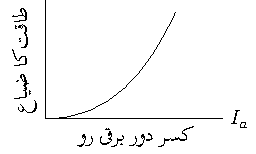
\includegraphics{figSynchronousShortCircuitedLoss}
\begin{tikzpicture}
%axis
\draw[] (0,0)--(3,0)node[right]{$ I_a$};
\draw[] node at (1.5,-0.3){\RL{کسر دور برقی رو}};
\draw[] (0,0)--(0,2)node[xshift=-0.35cm,rotate=90,pos=0.5]{\RL{ضیاع طاقت}};
%curves
\draw (0,0) to [out=0,in=-115] (2.2,1.8);
\end{tikzpicture}
\caption{کسر دور معاصر مشین میں ضیاع طاقت۔}
\label{شکل_معاصر_کسر_دور_ضیاع}
\end{figure}
\ابتدا{مثال}
ایک  \عددیء{75} کلو وولٹ-ایمپیئر،  \عددیء{415} وولٹ پر چلنے والی تین دوری معاصر مشین کے پورے (بناوٹی) برقی رو پر  کل کسر دور طاقت کا ضیاع  \عددیء{2.2} کلو واٹ ہے۔ اس مشین کی یک دوری موثر مزاحمت حاصل کریں۔

حل:\quad
یک دوری ضیاع  \عددیء{\tfrac{2200}{3}=\SI{733.33}{\watt}}  ہے ۔مشین کے پوری برقی رو درج ذیل ہو گا۔
\begin{align*}
\frac{75000}{\sqrt{3} V_{\textup{تار}}}=\SI{104.34}{\ampere}
\end{align*}
یوں مشین کی موثر مزاحمت درج ذیل ہو گی۔
\begin{align*}
R_a=\frac{733.33}{104.34^2}=\SI{0.067}{\ohm}
\end{align*}
\انتہا{مثال}
%
\ابتدا{مثال}
شکل \حوالہ{شکل_معاصر_کھلے_دور_بریلووین_خط}  میں \عددیء{500} وولٹ، \عددیء{50} ہرٹز، \عددیء{4} قطب، ستارہ، معاصر جنریٹر کا کھلے دور خط دکھایا گیا ہے۔اس جنریٹر کا معاصر امالہ \عددیء{0.1} اوہم اور قوی لچھے کی مزاحمت \عددیء{0.01} اوہم ہے۔پورے برقی بوجھ، \عددیء{0.92} تاخیری جزو طاقت\حاشیہب{lagging power factor} پر  جنریٹر \عددیء{1000} ایمپیئر فراہم کرتا ہے۔پورے بوجھ پر رگڑی ضیاع اور لچھے کی مزاحمت میں ضیاع کا مجموعہ \عددیء{30} کلو واٹ جبکہ قالبی ضیاع \عددیء{25} کلو واٹ ہے۔
\begin{itemize}
\item
جنریٹر کی رفتار معلوم کریں۔
\item
بے بوجھ جنریٹر کی سروں پر \عددیء{500} وولٹ برقی دباو کتنے میدانی برقی رو پر حاصل ہو گا؟
\item
اگر جنریٹر پر  \عددیء{0.92} تاخیری جزو طاقت، \عددیء{1000} ایمپیئر کا برقی بوجھ لادا جائے تب جنریٹر کے برقی سروں پر \عددیء{500} وولٹ برقرار رکھنے کے لئے کتنا میدانی برقی رو درکار ہو گا؟
\item
جنریٹر پورے بوجھ پر کتنی طاقت فراہم کر رہا ہے جبکہ اس کو محرک کتنی میکانی طاقت فراہم کر رہا ہے۔ان دو سے جنریٹر کی فی صد \اصطلاح{کارگزاری}\فرہنگ{کارگزاری}\حاشیہب{efficiency} تلاش کریں۔
\item
اگر جنریٹر سے یک دم برقی بوجھ ہٹایا جائے تو اس لمحہ اس کے برقی سروں پر کتنا برقی دباو ہو گا؟
\item
اگر جنریٹر پر \عددیء{1000} ایمپیئر  \عددیء{0.92}  پیش جزو طاقت کا بوجھ لادا جائے تو جنریٹر کے برقی سروں پر \عددیء{500} وولٹ برقرار رکھنے کے لئے کتنا میدانی برقی رو درکار ہو گا؟
\item
ان  \عددیء{1000} ایمپیئر تاخیری جزو طاقت اور پیش جزو طاقت بوجھوں میں کونسا بوجھ زیادہ میدانی برقی رو پر حاصل ہو گا؟ جنریٹر کس بوجھ سے زیادہ گرم ہو گا؟
\end{itemize}
%
\begin{figure}
\centering
%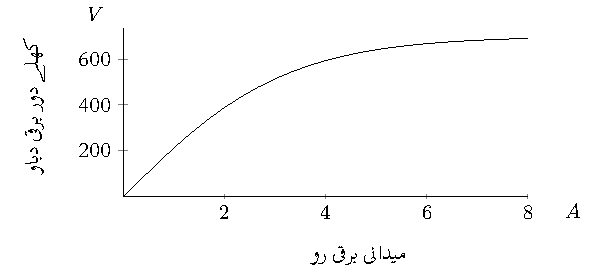
\includegraphics{figSynchronousOpenCircuitCharacteristicsBrillouinFunction}
\pgfmathsetmacro{\J}{0.5}
\pgfmathsetmacro{\k}{(2*\J+1)/(2*\J)}
\begin{tikzpicture}[
  declare function={
    kBJ(\x)= and(\x>-0.001, \x< 0.001)*(0)+or(\x<-0.001, \x>0.001)*(\k*(e^(\k*\x)+e^(-\k*\x))/(e^(\k*\x)-e^(-\k*\x))-1/(2*\J)*(e^(\x/(2*\J))+e^(-\x/(2*\J)))/(e^(\x/(2*\J))-e^(-\x/(2*\J))));
  }
]
\begin{axis}[yscale=0.5,
ymax=1.05,
  axis x line=middle, axis y line=middle,
 % ymin=-5, ymax=5, ytick={-5,...,5}, 
axis line style=-,
ylabel=$V$,
  %xmin=-5, xmax=5, xtick={-5,...,5}, 
xlabel=$A$,
xlabel style={below right,xshift=0.5cm},
ylabel style={above left,xshift=-0.2cm},
xtick={0.625,1.25,1.875,2.5},
xticklabels={$2$,$4$,$6$,$8$},
ytick={0.286,0.571,0.857},
yticklabels={200,400,600},
]
\addplot[domain=0:2.5]{kBJ(x)};
\end{axis}
\draw node at (4,-1){\RL{میدانی برقی رو}};
\draw node[rotate=90] at (-1.5,1.5){\RL{کھلا دور برقی دباو}};
\end{tikzpicture} 
\caption{کھلا دور خط۔}
\label{شکل_معاصر_کھلے_دور_بریلووین_خط}
\end{figure}
حل:
\begin{itemize}
\item
\عددیء{f_e=\tfrac{P}{2} f_m} سے \عددیء{f_m=\tfrac{2}{4} \times 50=25} چکر فی سیکنڈ یا \عددیء{25 \times 60=1500} چکر فی منٹ حاصل ہوتا ہے۔
\item
شکل \حوالہ{شکل_معاصر_کھلے_دور_بریلووین_خط}  سے  \عددیء{500}  وولٹ کے لئے درکار میدانی برقی رو تقریباً \عددیء{2.86} ایمپیئر پڑھا جاتا  ہے۔
\item
ستارہ برقی دباو کے تعلق \عددیء{V_{\textup{تار}}=\sqrt{3} V_{\textup{یکدوری}}} سے \عددیء{V_{\textup{یکدوری}}=\tfrac{500}{\sqrt{3}}=289}  وولٹ حاصل ہوتا ہے۔ستارہ جوڑ میں یک دوری برقی رو اور تار برقی رو برابر ہوتے ہیں۔جزو طاقت کو ستارہ یک دوری برقی دباو کے نسبت سے بیان کیا جاتا ہے۔چونکہ \عددیء{\cos^{-1} 0.92=23.07\degree} ہے لہٰذا اگر برقی سروں پر دباو \عددیء{289 \phase {0 \degree}} لکھا جائے تب تاخیری دوری برقی رو \عددیء{1000\phase {-23.07 \degree}}  لکھا جائے گا۔یوں شکل \حوالہ{شکل_معاصر_جنریٹر_کا_مساوی_دور} یا مساوات \حوالہ{مساوات_معاصر_جنریٹر_دوری_سمتیہ_مساوات} سے اندرونی پیدا یک دوری برقی دباو
\begin{align*}
\hat{E}_a&=\hat{V}_{a}+\hat{I}_a \left(R_a+j X_s \right)\\
&= 289\phase{0 \degree}+1000 \phase {-23.07 \degree} ( 0.01 +j 0.1)\\
&=349\phase{14.6 \degree}
\end{align*}
حاصل ہو گا جس سے اندرونی پیدا تار برقی دباو \عددیء{\sqrt{3} \times 349=604} وولٹ حاصل ہوتا ہے۔شکل \حوالہ{شکل_معاصر_کھلے_دور_بریلووین_خط} سے اتنے دباو کے لئے  \عددیء{\SI{4.1}{\ampere}} میدانی برقی رو پڑھا جاتا ہے۔
\item
جنریٹر اس صورت میں
\begin{align*}
p&=\sqrt{3} \hat{V}_{a} \cdot \hat{I}_a\\
&=\sqrt{3} \times 500 \times 1000 \times 0.92\\
&=\SI{796743}{\watt}
\end{align*}
فراہم کر رہا ہے جبکہ محرک 
\begin{align*}
p_m&=796.743+30+25=\SI{851.74}{\kilo \watt}
\end{align*}
فراہم کر رہا ہے لہٰذا اس جنریٹر کی کارگزاری \عددیء{\eta = \tfrac{796.743}{851.74} \times 100=93.54 \%} ہے۔
\item
جنریٹر سے یک دم برقی بوجھ ہٹانے کے  لمحہ پر جنریٹر کے برقی سروں پر \عددیء{604}  وولٹ برقی دباو ہو گا۔
\item
پیش جزو طاقت کی صورت میں
\begin{align*}
\hat{E}_a&=\hat{V}_{a}+\hat{I}_a \left(R_a+j X_s \right)\\
&= 289\phase{0 \degree}+1000 \phase {23.07 \degree} ( 0.01 +j 0.1)\\
&=276\phase{20.32 \degree}
\end{align*}
ہو گا جس سے اندرونی پیدا تار برقی دباو \عددیء{\sqrt{3} \times 276=478} وولٹ حاصل ہوتا ہے۔شکل \حوالہ{شکل_معاصر_کھلے_دور_بریلووین_خط} سے اتنے دباو کے لئے  \عددیء{\SI{2.7}{\ampere}} میدانی برقی رو درکار ہو گا۔
\item
تاخیری جزو طاقت کے بوجھ پر جنریٹر کو زیادہ میدانی برقی رو درکار ہے۔میدانی لچھے کی مزاحمت میں اس کی وجہ سے زیادہ برقی طاقت ضائع ہو گی اور جنریٹر  زیادہ گرم ہو گا۔
\end{itemize}
\انتہا{مثال}
%
\ابتدا{مثال}
ایک \عددیء{415} وولٹ، \عددیء{40} کلو وولٹ-ایمپیئر، ستارہ، \عددیء{0.8} جزو طاقت، \عددیء{50} ہرٹز پر چلنے والی معاصر موٹر کا معاصر امالہ \عددیء{2.2} اوہم  ہے جبکہ اس کی مزاحمت قابل نظرانداز ہے۔اس کی رگڑ اور لچھوں کی مزاحمت میں طاقت کا ضیاع ایک کلو واٹ جبکہ قالبی ضیاع \عددیء{800} واٹ ہے۔یہ موٹر \عددیء{12.2}  کلوواٹ میکانی بوجھ سے لدی  ہے اور یہ \عددیء{0.8}  پیش جزو طاقت   پر چل رہی ہے۔یاد رہے کہ معاصر امالہ مشین کو ستارہ نما تصور کرتے ہوئے حاصل کیا جاتا ہے۔ 
\begin{itemize}
\item
اس کا دوری سمتیہ بنائیں۔تار کا برقی رو \عددیء{\hat{I}_t} اور قوی لچھے کا برقی رو  \عددیء{\hat{I}_a} حاصل کریں۔موٹر کا اندرونی ہیجانی برقی دباو \عددیء{\hat{E}_a} حاصل کریں۔
\item
میدانی برقی رو کو بغیر تبدیل کئے،  میکانی بوجھ آہستہ آہستہ بڑھا کر دگنا کیا جاتا ہے۔اس صورت میں موٹر کا رد عمل دوری سمتیہ سے واضح کریں ۔
\item
اس دگنے میکانی بوجھ پر قوی لچھے  کا برقی رو،  تار کا برقی رو  اور موٹر کا اندرونی ہیجانی برقی دباو حاصل کریں۔موٹر کا جزو طاقت بھی حاصل کریں۔
\end{itemize}

حل:
\begin{itemize}
\item
ستارہ جڑی موٹر کے سروں پر یک دوری برقی دباو \عددیء{\tfrac{415}{\sqrt{3}}=\SI{239.6}{\volt}}  ہو گا جسے صفر زاویہ پر تصور کرتے ہوئے برقی رو کا زاویہ بیان کیا جاتا ہے۔یوں \عددیء{\hat{V}_{sa}=239.6\phase {0\degree}} لکھا جائے گا۔جزو طاقت \عددیء{0.8} زاویہ  \عددیء{36.87\degree} کو ظاہر کرتا ہے۔ یوں تار برقی رو کا \اصطلاح{پیش} زاویہ یہی ہو گا۔موٹر کو مہیا برقی طاقت اس کی میکانی طاقت اور طاقت کے ضیاع کے برابر ہو گی
\begin{align*}
\SI{12200}{\watt}+\SI{1000}{\watt}+\SI{800}{\watt}=\SI{14000}{\watt}
\end{align*}
جس  کے لئے درکار تار کا برقی رو درج ذیل ہو گا۔ 
\begin{align*}
I_t&=\frac{p}{\sqrt{3} V_{t} \cos \theta}\\
&=\frac{\num{14000}}{\sqrt{3} \times 415 \times 0.8}\\
&=\SI{24.346}{\ampere}
\end{align*}
ستارہ جڑی موٹر کے قوی لچھے کا برقی رو تار کے برقی رو کے برابر ہو گا۔یوں برقی رو کا زاویہ شامل کرتے ہوئے اسے 
\begin{align*}
\hat{I}_a=\hat{I}_t=24.346 \phase {36.87 \degree}
\end{align*}
لکھا جا سکتا ہے۔

موٹر کا اندرونی یک دوری ہیجانی برقی دباو موٹر کے مساوی دور شکل \حوالہ{شکل_معاصر_موٹر_کا_مساوی_دور}  کی مدد سے درج ذیل ہو گا۔
\begin{align*}
\hat{E}_a&=\hat{V}_{a,s}- j X_s \hat{I}_a\\
&=239.6 \phase{0\degree}-j 2.2 \times 24.346 \phase{36.87\degree}\\
&=276 \phase{-8.96\degree}
\end{align*}
اس تمام صورت حال کو شکل \حوالہ{شکل_معاصر_بار_بردار_جنریٹر_مثال}  میں دوری سمتیات کی مدد سے دکھایا گیا ہے۔
\begin{figure}
\centering
%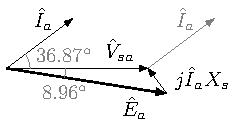
\includegraphics{figSynchronousLoadedGeneratorExample}
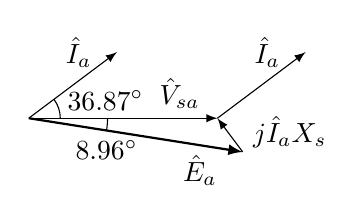
\begin{tikzpicture}
\draw[-latex] (0,0)--++(2.396,0)node[pos=0.8,above]{$\hat{V}_{sa}$}coordinate(vTip);
\draw[-latex](0,0)--++(36.87:1.4)node[left,xshift=-0.2cm]{$\hat{I}_a$};
\draw [] (0.4,0) arc (0:36.87:0.4);
\draw [] node at (13:1){$36.87^\circ$};
\draw[-latex] (vTip)--++(36.87:1.4)node[left,xshift=-0.2cm]{$\hat{I}_a$};
\draw[latex-] (vTip)--++(-53.13:0.5356)node[pos=0.4,right,xshift=0.2cm]{$j \hat{I}_a X_s$}coordinate(loadTip);
\draw[-latex,thick] (0,0)--(loadTip)node[below,pos=0.8]{$\hat{E}_a$};
\draw[](1,0) arc (0:-8.96:1)node[below]{$8.96^\circ$};
\end{tikzpicture}%
\caption{بوجھ بردار معاصر موٹر۔}
\label{شکل_معاصر_بار_بردار_جنریٹر_مثال}
\end{figure}
%
\item
میکانی بوجھ بڑھنے سے موٹر کو زیادہ برقی طاقت درکار ہو گی۔ یہ اس صورت ممکن ہو گا جب موٹر کے قوی لچھے کا برقی رو بڑھ سکے۔میدانی برقی رو معین ہونے کی وجہ سے موٹر کے اندرونی ہیجانی برقی دباو \عددیء{\hat{E}_a} کی مطلق قیمت  تبدیل نہیں ہو سکتی البتہ اس کا زاویہ تبدیل ہو سکتا ہے۔موٹر  \عددیء{\hat{E}_a}  کی مطلق قیمت تبدیل کئے بغیر  برقی سروں پر لاگو برقی دباو  \عددیء{\hat{V}_a}  اور \عددیء{\hat{E}_a}  کے بیچ زاویہ بڑھا کر قوی لچھے کا برقی رو اور یوں حاصل برقی طاقت بڑھائے گا۔ایسا شکل \حوالہ{شکل_معاصر_بار_بڑھانے_کا_اثر}  میں دکھایا گیا ہے جہاں  \عددیء{\hat{E}_a} دوری سمتیہ کی نوک  گول دائرہ پر رہتی ہے۔یوں اس کا طول تبدیل نہیں ہوتا۔زاویہ بڑھنے سے \عددیء{\abs{j\hat{I}_a X_s}} بڑھتا ہے۔چونکہ \عددیء{X_s} نہیں بڑھ رہا لہٰذا درحقیقت قوی لچھے کا برقی رو بڑھ گیا ہے۔زیادہ بوجھ کی صورت حال کو نقطہ دار دکھایا گیا ہے۔
\begin{figure}
\centering
%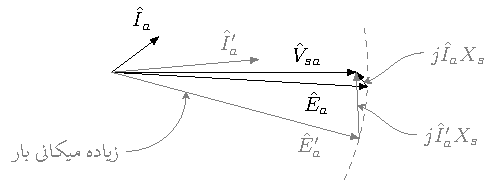
\includegraphics{figSynchronousLoadedGeneratorIncreasingLoad}
\begin{tikzpicture}
\draw[-latex] (0,0)--++(4.14,0)node[pos=0.8,above]{$\hat{V}_{sa}$}coordinate(vTip);
\draw[-latex](0,0)--++(36.87:1)node[above left]{$\hat{I}_a$};
%
\draw[-latex] (0,0)--(-3.266:4.34)coordinate(genVtip)node[below,pos=0.8]{$\hat{E}_a$};
\draw[-latex] (genVtip)--(vTip)coordinate[pos=0.3](load);
\draw[gray] (load) to [out=20,in=180] ++(1,0.5) node[right,black]{$j \hat{I}_a X_s$};
%
\draw[] (10:4.34) arc (10:-25:4.34);
%
\draw[-latex,dashed](0,0)--++(-15:4.34)coordinate(genVtipA)node[below,pos=0.8]{$\hat{E}_a'$}coordinate[pos=0.3](greaterLoad);
\draw[-latex,dashed] (genVtipA)--(vTip)coordinate[pos=0.5](loadA);
\draw[-latex,dashed](0,0)--(5:2.5)node[pos=0.8,above]{$\hat{I}_a'$};
\draw[gray] (loadA)++(0.03,0) to [out=-20,in=180] ++(1,-0.5) node[right,black]{$j \hat{I}_a' X_s$};
\draw[] (greaterLoad)node[pin=-135:{\RL{زیادہ میکانی بوجھ}}]{};
\end{tikzpicture}%
\caption{بوجھ بڑھنے کا اثر۔}
\label{شکل_معاصر_بار_بڑھانے_کا_اثر}
\end{figure}
%
\item
دگنی میکانی بوجھ پر موٹر کو کل \عددیء{24400+800+1000=26200}  واٹ یا \عددیء{26.2}  کلو واٹ برقی طاقت درکار ہے۔مساوات \حوالہ{مساوات_معاصر_سائن_خصوصیات}  کی مدد سے درج ذیل ہو گا۔
\begin{align*}
\sigma&=\sin^{-1} \left(\frac{p X_s}{3 V_a E_a} \right)=\sin^{-1} \left(\frac{26200 \times 2.2}{3\times 239.6 \times 276} \right)=16.89\degree
\end{align*}
یوں موٹر کا اندرونی ہیجانی برقی دباو \عددیء{276 \phase{-16.89\degree}} ہو گا اور قوی لچھے کا برقی رو درج ذیل ہو گا۔
\begin{align*}
\hat{I}_a&=\frac{\hat{V}_a-\hat{E}_a}{j X_s}\\
&=\frac{239\phase{0\degree}-276\phase{-16.89\degree}}{j 2.2}\\
&=38\phase{17.4\degree}
\end{align*}
ستارہ جوڑ کی وجہ سے \عددیء{\hat{I}_t} بھی اتنا ہی ہو گا۔پیش جزو طاقت \عددیء{\cos 17.4 \degree=0.954} ہے۔
\end{itemize}
\انتہا{مثال}
